\chapter{RAG Chatbot}

\section{Obiettivi Chatbot e scelte tecniche}
Durante la mia esperienza di tirocinio, mi sono occupato dello sviluppo di un chatbot con l'obiettivo di fornire all'azienda uno strumento open source capace di rispondere alle domande utilizzando dati specifici relativi all'azienda.
L'idea iniziale era quella di eseguire un fine-tuning utilizzando un modello di linguaggio open source e sviluppare un'applicazione che permettesse agli utenti di scrivere domande e ricevere risposte. Tuttavia, questo approccio richiedeva una grande quantità di dati e risorse computazionali, come GPU e almeno 16 o più GB di RAM, per effettuare l'addestramento del modello sul dataset personalizzato.
In conclusione, è stata scelta la soluzione di un chatbot basato su un sistema RAG. Questa scelta ha permesso di salvare i documenti come vettori in un database e di utilizzare un retriever per fornire conoscenza aggiuntiva al modello di linguaggio selezionato.

\section{Architettura del sistema}

\subsection{Componenti principali}
Il sistema è composto da un'applicazione Flutter che gestisce le operazioni di interazione con l'utente e da un server Python che rimane costantemente in ascolto per ricevere le richieste dell'utente tramite l'applicazione.

\subsection{Python Server}
Il server è un'applicazione Flask scritta in Python che resta in ascolto per richieste HTTP e svolge diverse funzioni in base al tipo di richiesta ricevuta. Il server gestisce l'elaborazione dei documenti e delle domande inviate dall'applicazione Flutter, generando rispettivamente il contesto e la risposta. Inoltre, l'applicazione Flutter contatta il server per ottenere la lista dei contesti archiviati per un determinato utente all'interno del database gestito dal server.

\subsection{Applicazione Flutter}
\subsubsection{Flutter}
Flutter è un framework open-source creato da Google per la creazione di interfacce native per iOS, Android, Linux, macOS, Windows e con la versione 1.9 è stato introdotto il supporto per le applicazioni web e per siti statici scritti in linguaggio Dart.
Flutter ha riscosso particolare successo grazie alla sua capacità di essere cross-platform, permettendo lo sviluppo di applicazioni per tutti i principali sistemi operativi utilizzando il linguaggio Dart.

\subsubsection{Pagina di login}
La pagina di login permette all'utente di accedere alla piattaforma tramite credenziali.
La Figura \ref{fig:login-page} illustra la pagina di login. Per verificare l'esistenza di un utente, utilizziamo Firebase Console, che consente di memorizzare le informazioni dell'utente in un database al momento della registrazione. La Figura \ref{fig:invalid_credentials} rappresenta l'errore che viene generato come risultato dell'inserimento di credenziali errate o inesistenti, mentre la Figura \ref{fig:empty_field} mostra l'esito del tentativo di login quando uno o più campi vengono lasciati vuoti.
\begin{figure}[H]
	\centering
	\begin{subfigure}{.5\textwidth}
		\centering
		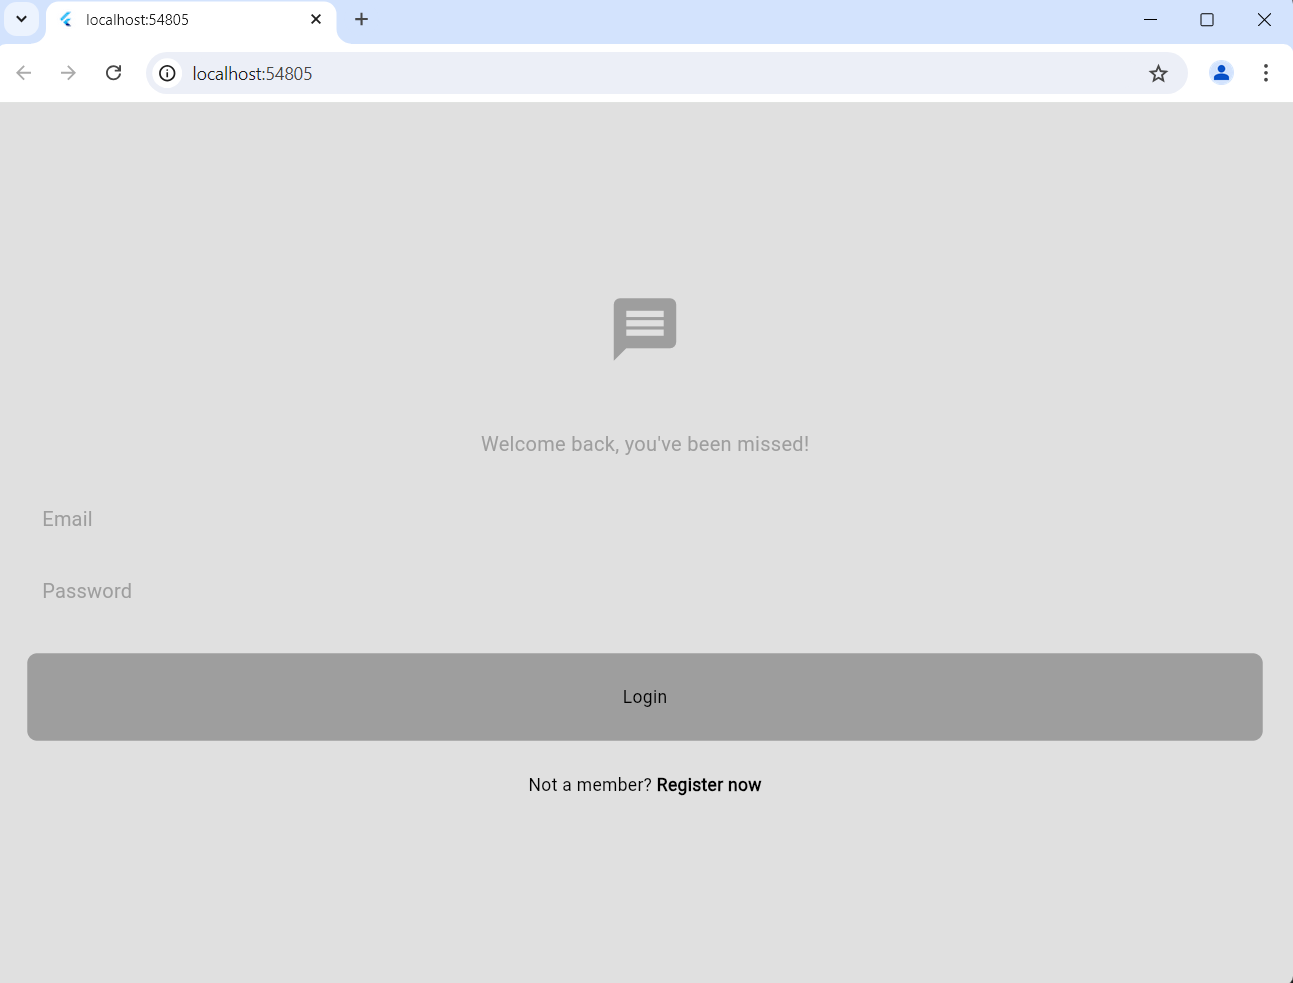
\includegraphics[width=0.45\linewidth]{Immagini/login_page.png}
		\caption{Pagina di login vuota\newline}
		\label{fig:login-page}
	\end{subfigure}%
	\begin{subfigure}{.5\textwidth}
		\centering
		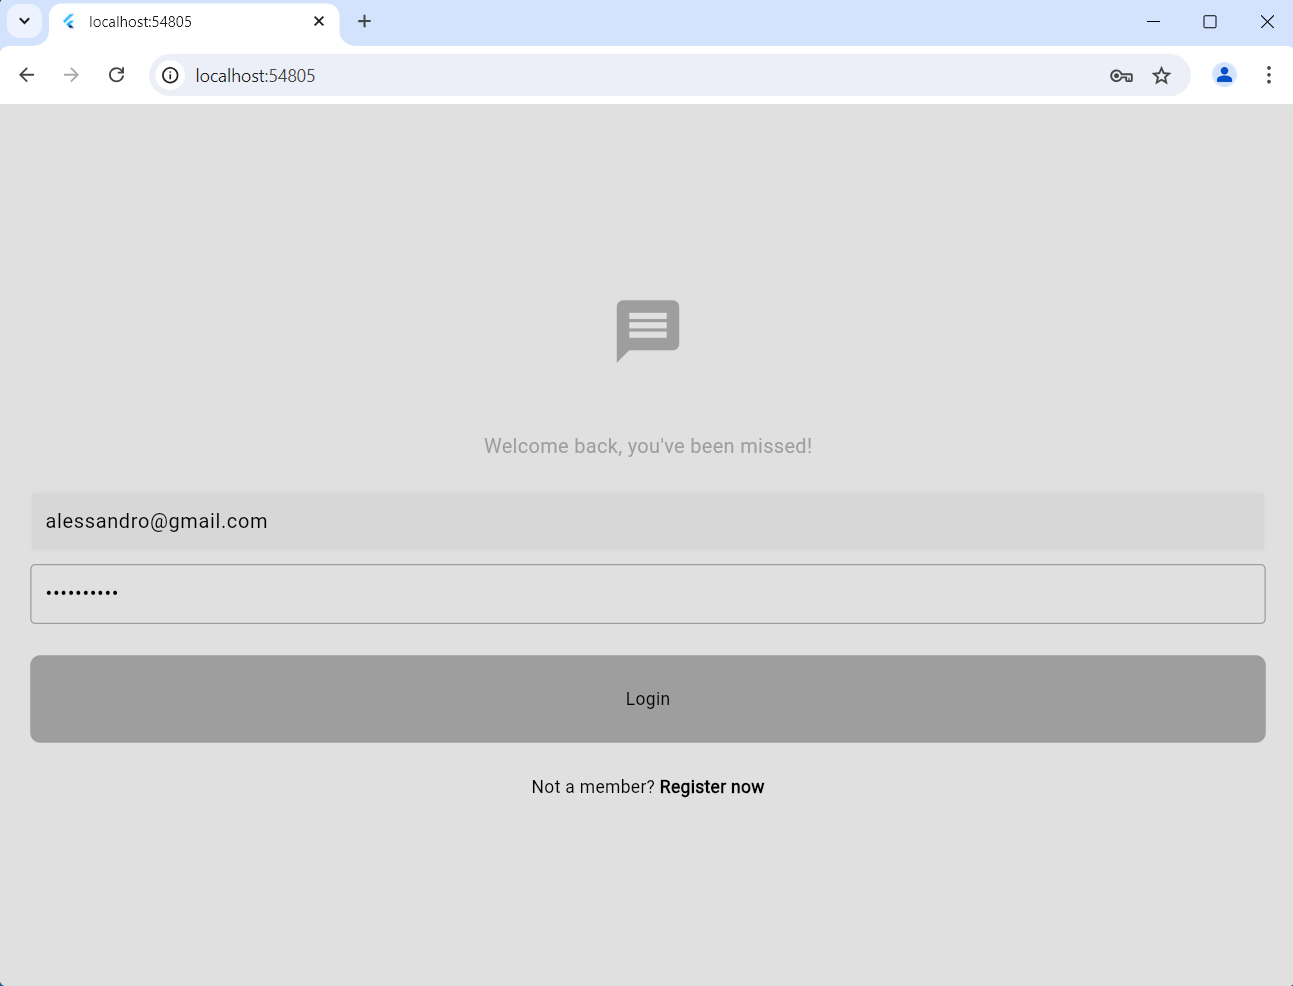
\includegraphics[width=0.45\linewidth]{Immagini/login_page_credentials.png}
		\caption{Pagina di login con credenziali inserite\newline}
		\label{fig:credential_login_page}
	\end{subfigure}
	\begin{subfigure}{.5\textwidth}
		\centering
		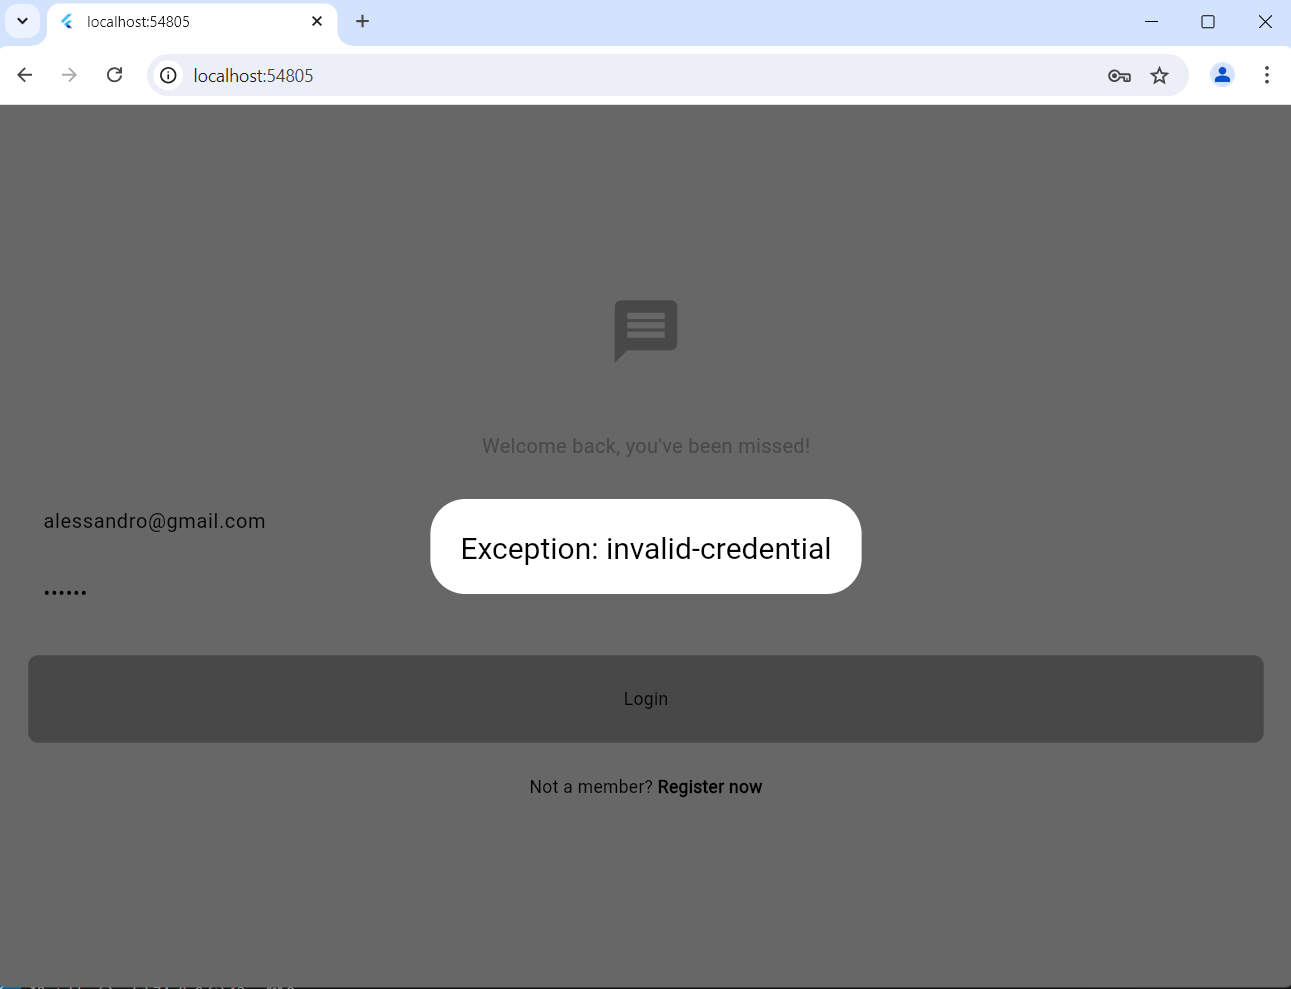
\includegraphics[width=0.45\linewidth]{Immagini/invalid_credentials.png}
		\caption{Errore dopo aver inserito credenziali invalide\newline}
		\label{fig:invalid_credentials}
	\end{subfigure}%
        \begin{subfigure}{.5\textwidth}
		\centering
		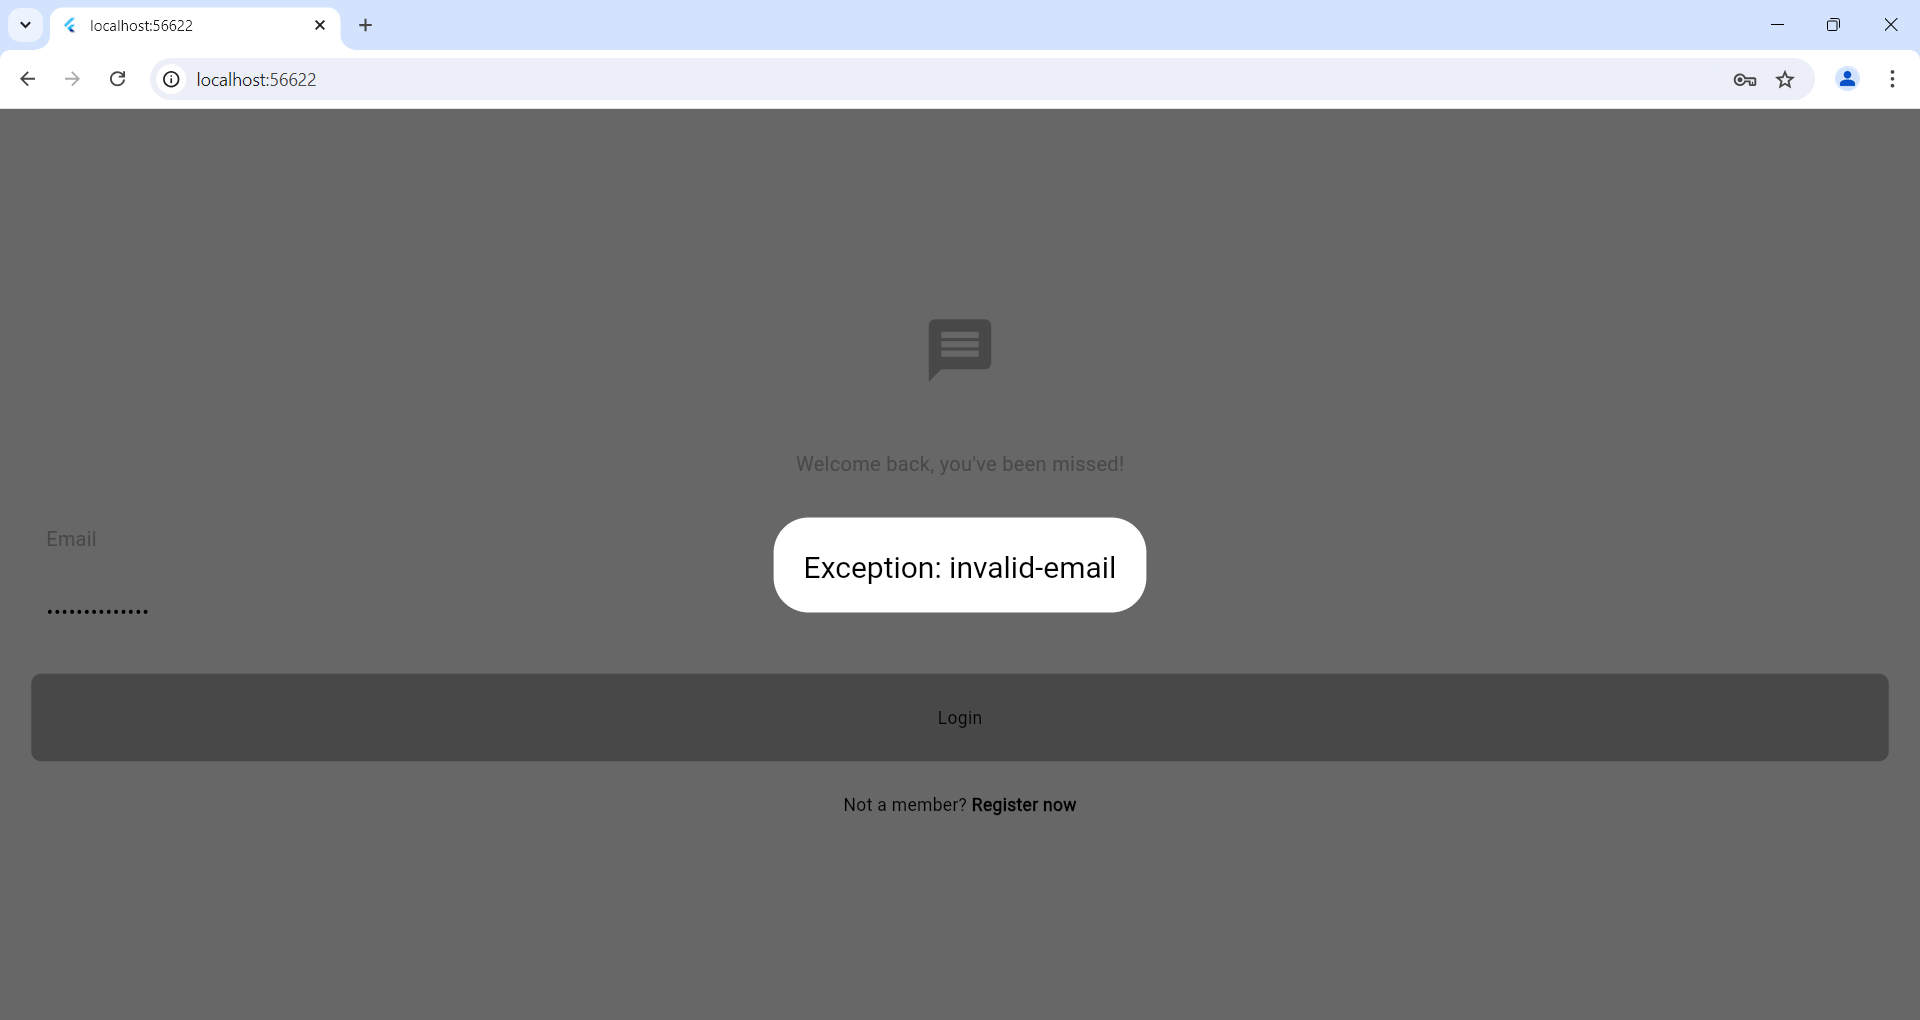
\includegraphics[width=0.45\linewidth]{Immagini/login_page_empty_field.png}
		\caption{Errore dopo aver lasciato un campo vuoto\newline}
		\label{fig:empty_field}
	\end{subfigure}%
	\caption{Pagina di login}
\end{figure}

\subsubsection{Pagina di registrazione}
La pagina di registrazione permette a un nuovo utente di creare un account utilizzando le proprie credenziali. Questo gli consentirà di accedere in modo sicuro e autonomo alla piattaforma in futuro. La registrazione risulta essere di fondamentale importanza poiché ad ogni utente viene assegnato un User-ID univoco, che verrà utilizzato dal server Python per estrarre i vettori contenenti i dati dei documenti salvati, che successivamente saranno forniti come contesto al chatbot. La figura \ref{fig:register_page} mostra la pagina di registrazione dell' applicazione.
\begin{figure}[ht]
	\centering
	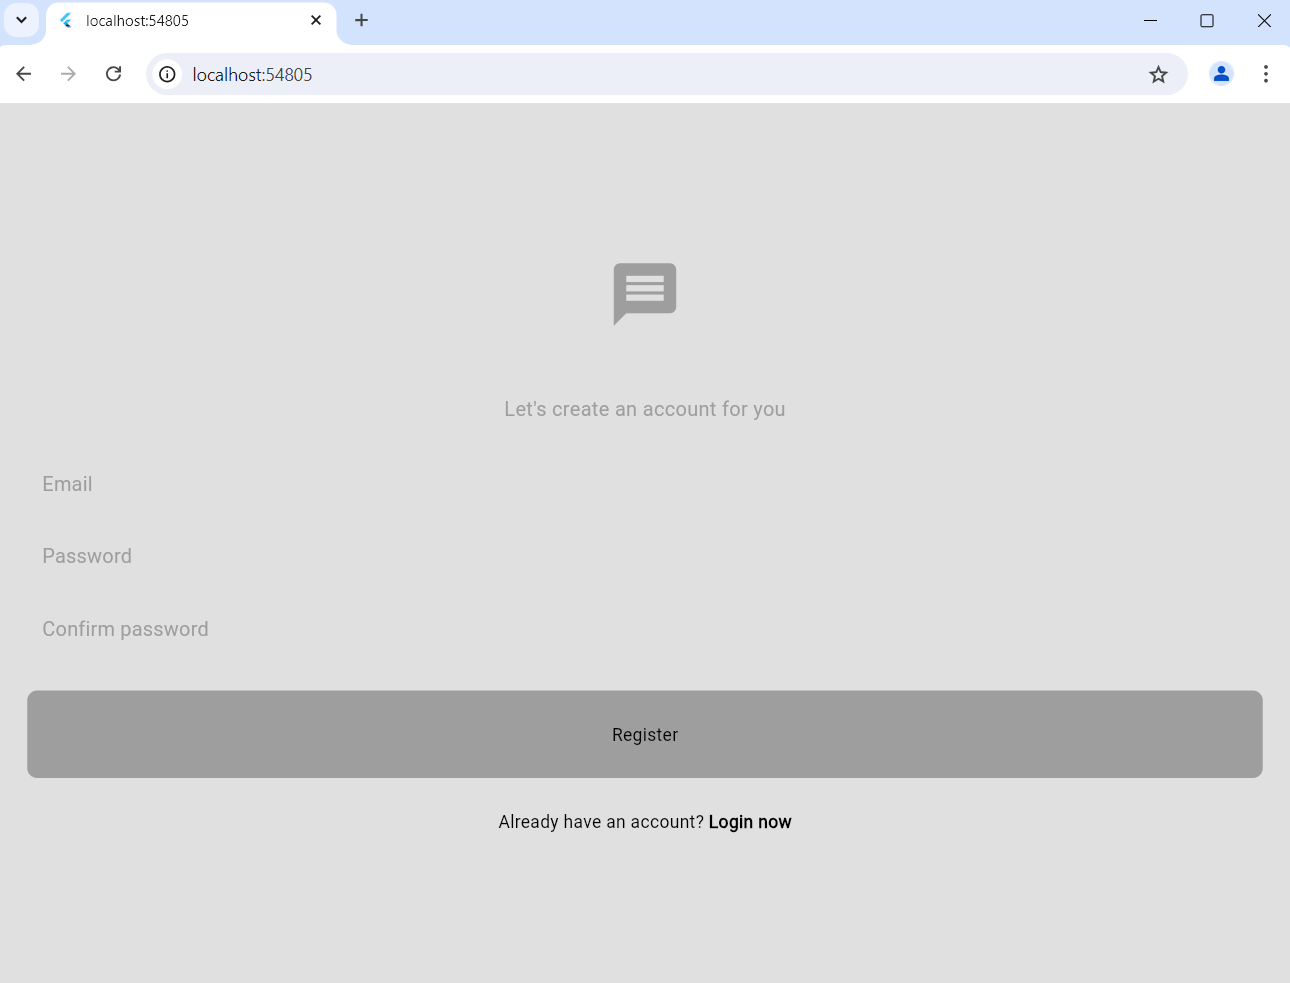
\includegraphics[width=0.3\textwidth]{Immagini/register_page.png}
	\caption{Pagina di registrazione dell'applicazione}
	\label{fig:register_page}
\end{figure}

\subsubsection{HomePage}
La Homepage consente all'utente di scegliere tra diverse modalità: Chatbot, MailBot, SpeechBot e DocUploader. Le prime tre opzioni rappresentano diverse tipologie di chatbot, mentre l'ultima permette di salvare nuovi contesti. Dopo il log in, l'applicazione invia una richiesta HTTP al server Python, che restituisce la lista di tutti i contesti precedentemente salvati dall'utente.
La Figura \ref{fig:home-page} mostra la HomePage dell'applicazione, mentre la Figura \ref{fig:window-home-page} illustra il menu a tendina che consente all'utente di effettuare il logout o modificare le impostazioni.
\begin{figure}[H]
	\centering
	\begin{subfigure}{.5\textwidth}
		\centering
		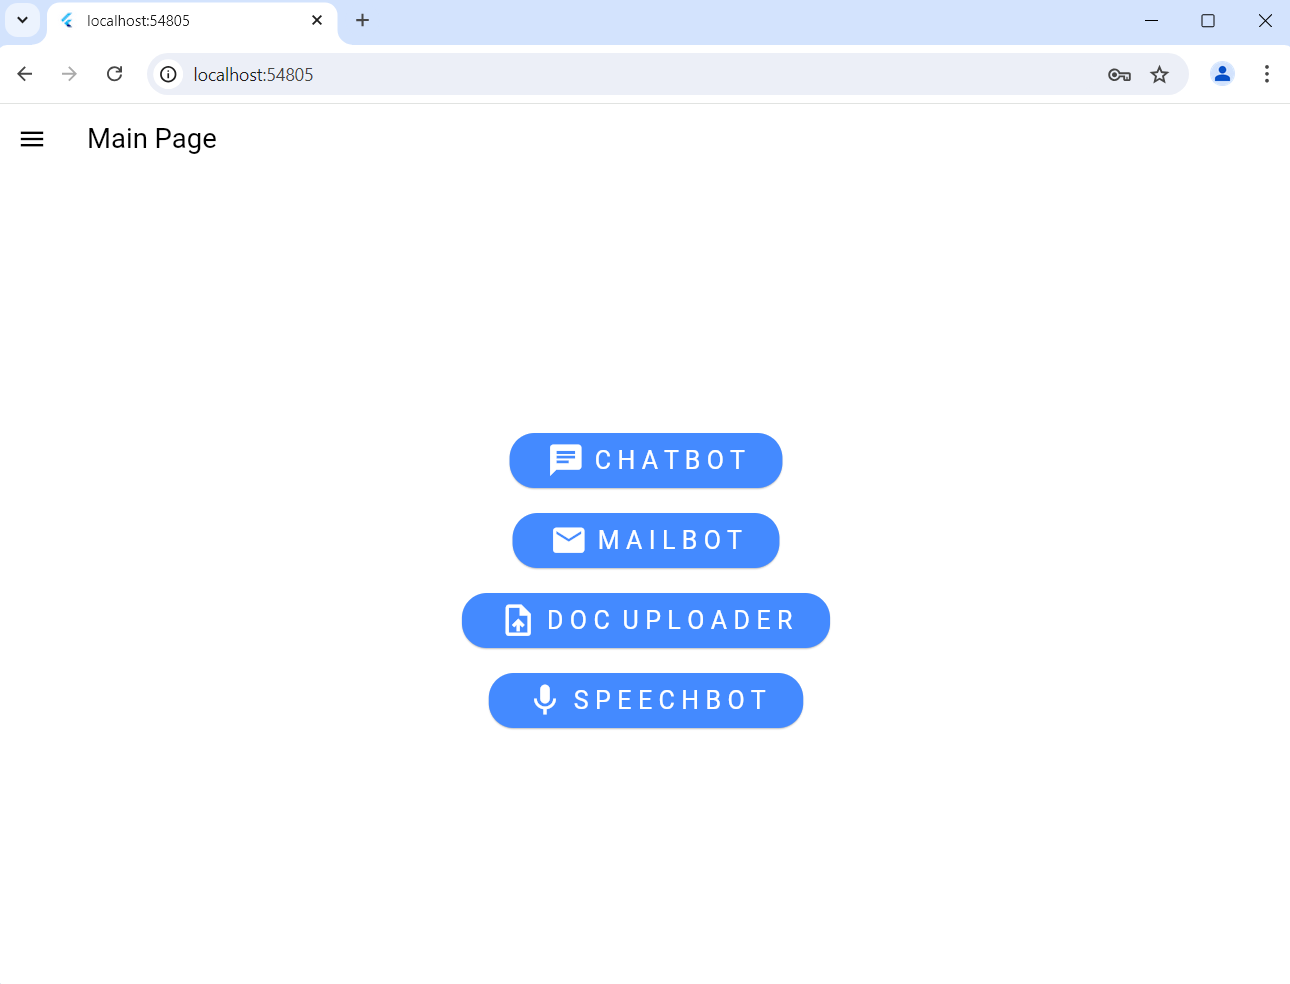
\includegraphics[width=0.45\linewidth]{Immagini/home_page.png}
		\caption{HomePage\newline}
		\label{fig:home-page}
	\end{subfigure}%
	\begin{subfigure}{.5\textwidth}
		\centering
		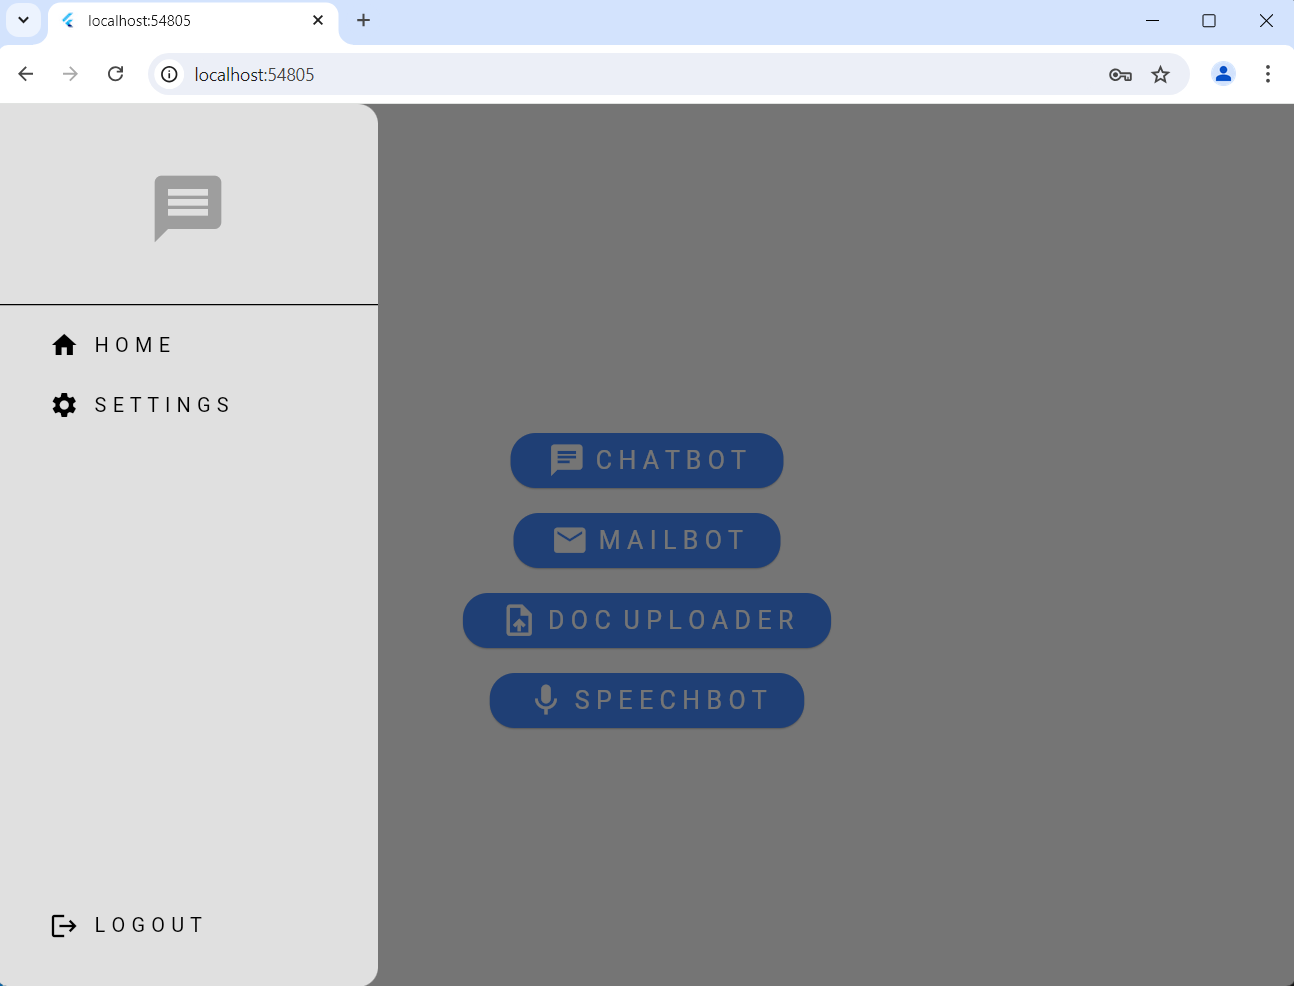
\includegraphics[width=0.45\linewidth]{Immagini/home_page_window.png}
		\caption{Tendina della HomePage\newline}
		\label{fig:window-home-page}
	\end{subfigure}
	\caption{HomePage dell'applicazione}
\end{figure}

\subsubsection{MailBot}
Il MailBot consente all'utente di inserire la propria email e la domanda, permettendo al server Python di inviare la risposta direttamente tramite posta elettronica. Questo sistema offre all'utente la comodità di inviare la propria domanda e ricevere la risposta via email, senza la necessità di attendere davanti all'applicazione.
Attraverso una richiesta HTTP, l'applicazione trasmette l'email e la domanda al server Python, il quale elabora la richiesta e utilizza il package `smtplib` per inviare la risposta all'indirizzo email fornito.
La figura \ref{fig:mailbot} illustra l'interfaccia della pagina del MailBot. Sulla destra è presente un'area che consente all'utente di selezionare il contesto necessario al Bot per fornire la risposta.
\begin{figure}[ht]
	\centering
	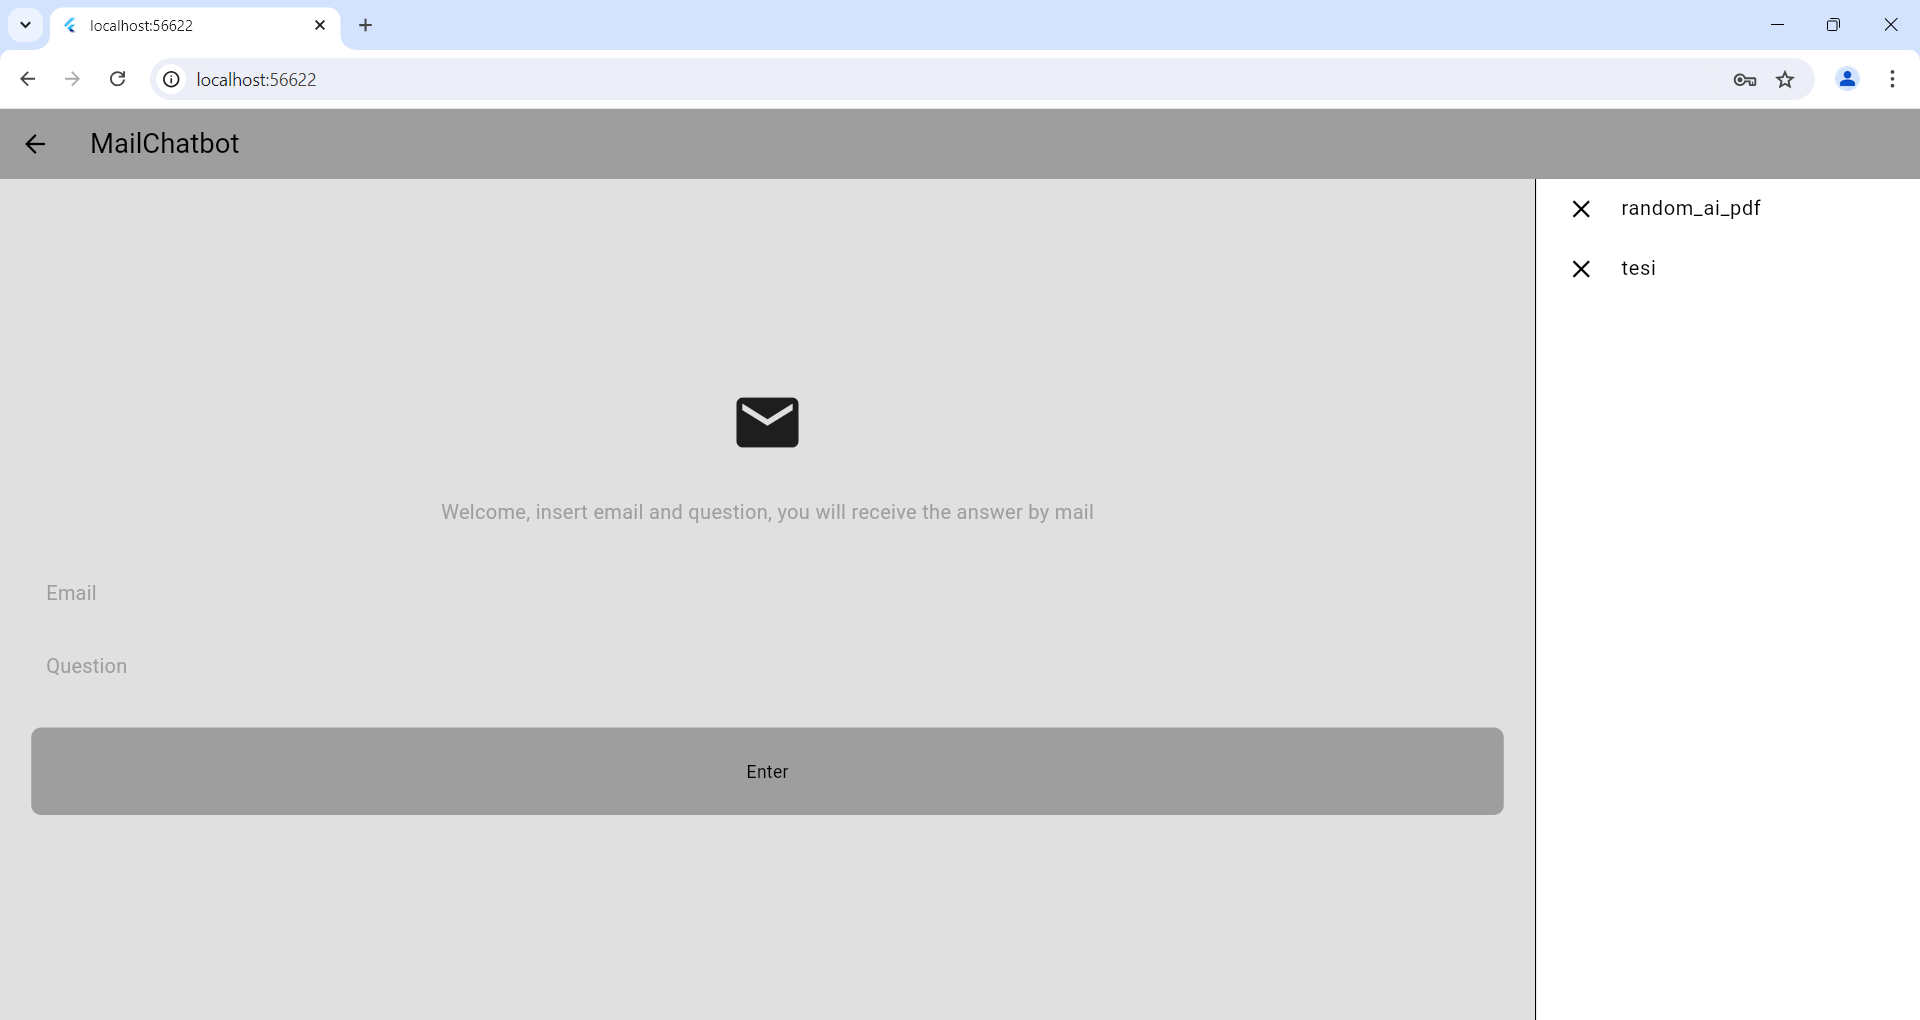
\includegraphics[width=0.3\textwidth]{Immagini/mailbot.png}
	\caption{Pagina del MailBot dell'applicazione}
	\label{fig:mailbot}
\end{figure}

\subsubsection{DocUploader}
La pagina di DocUploader consente all'utente di creare nuovi contesti tramite il caricamento di documenti.
La figura \ref{fig:doc_uploader_page} illustra l'interfaccia della pagina permettendo di scegliere tra due modalità: PdfUploader e HTMLPageUploader.
\begin{figure}[ht]
	\centering
	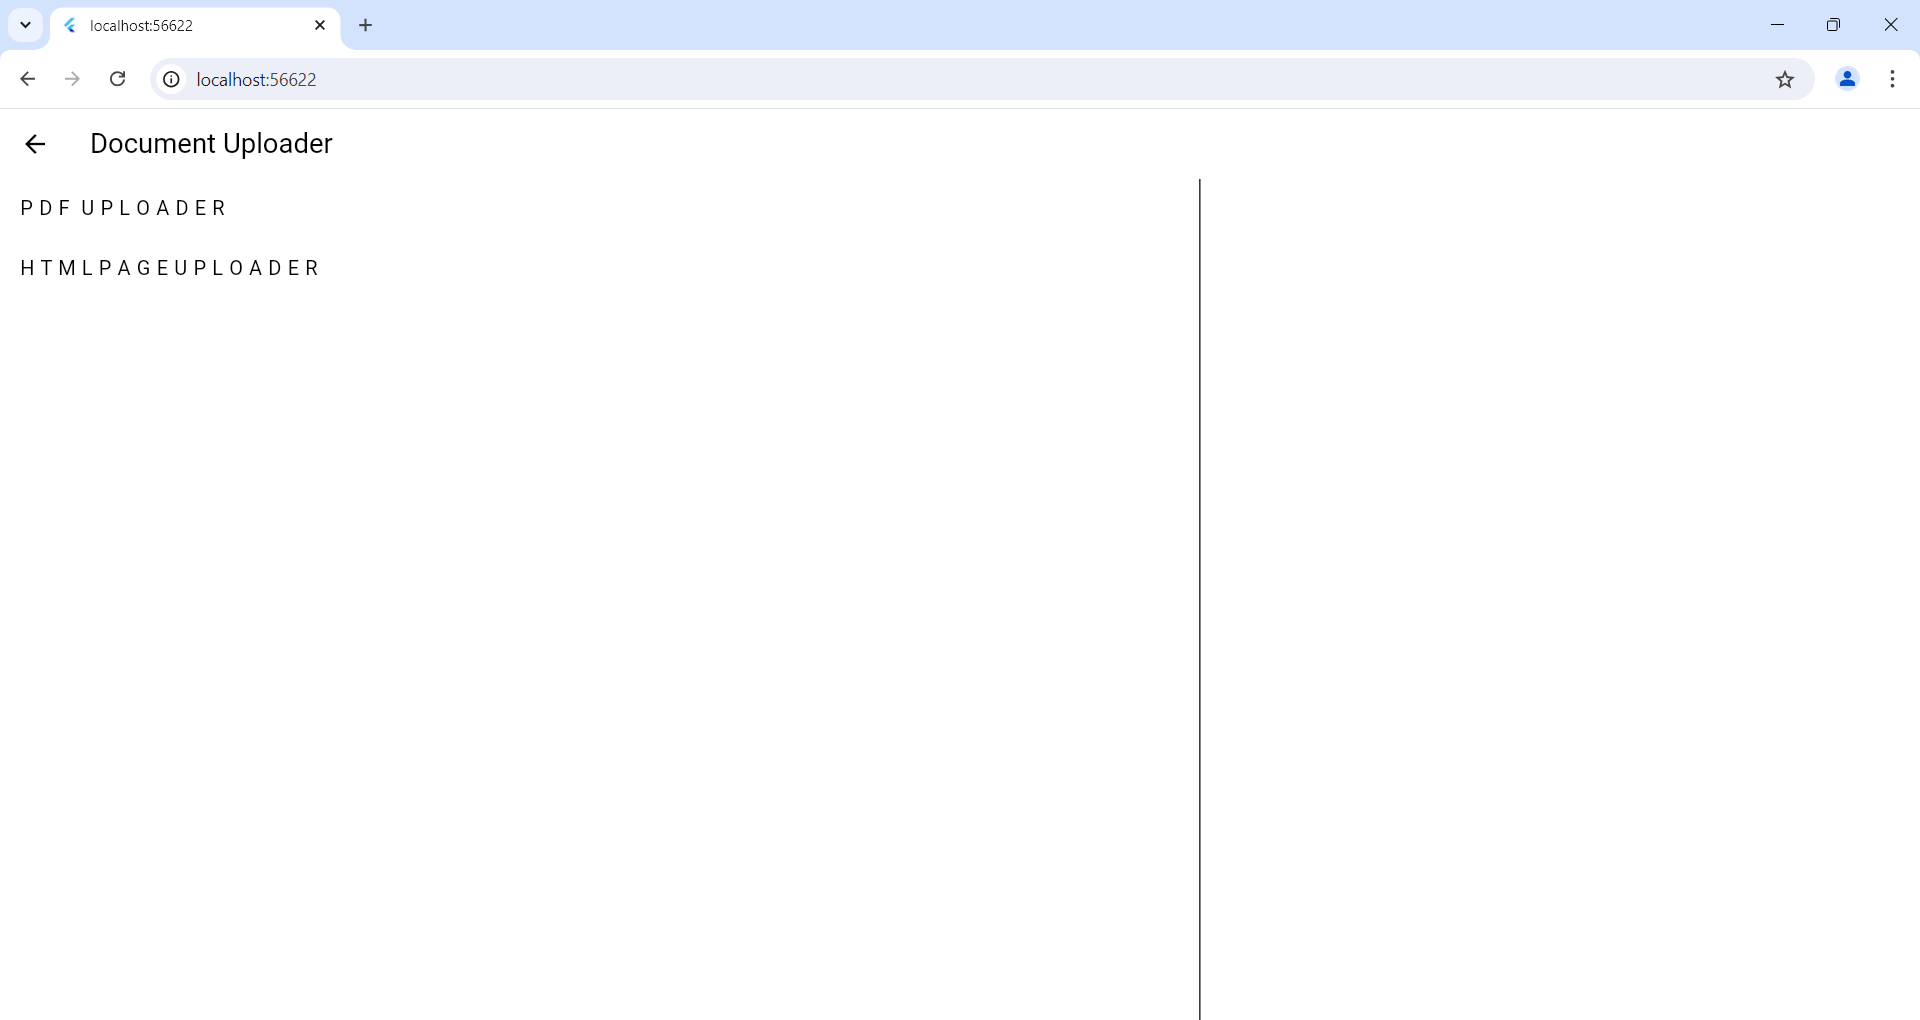
\includegraphics[width=0.3\textwidth]{Immagini/doc_uploader_page.png}
	\caption{Pagina del Doc Uploader dell'applicazione}
	\label{fig:doc_uploader_page}
\end{figure}

La figura \ref{fig:pdfs_page} illustra come l'utente possa creare un nuovo contesto basato su un documento PDF. L'applicazione offre un pulsante per il caricamento dei documenti PDF e un campo per inserire il nome del contesto, come mostrato nella figura \ref{fig:context-making}. Una volta che il pulsante "Process PDFs" viene premuto, l'applicazione invia una richiesta HTTP al server Python, includendo i byte del file PDF e una stringa contenente il nome del contesto.
Il server, ricevuta la richiesta, estrae i dati necessari, suddivide i documenti in segmenti (chunks) e utilizza un modello di embedding per creare un vettore, che sarà successivamente inserito nel database dei vettori associato all'utente specifico. Al termine del processo, l'utente riceve una notifica dell'avvenuta operazione, come illustrato nella figura \ref{fig:pdf_success}.
\begin{figure}[H]
	\centering
	\begin{subfigure}{.5\textwidth}
		\centering
		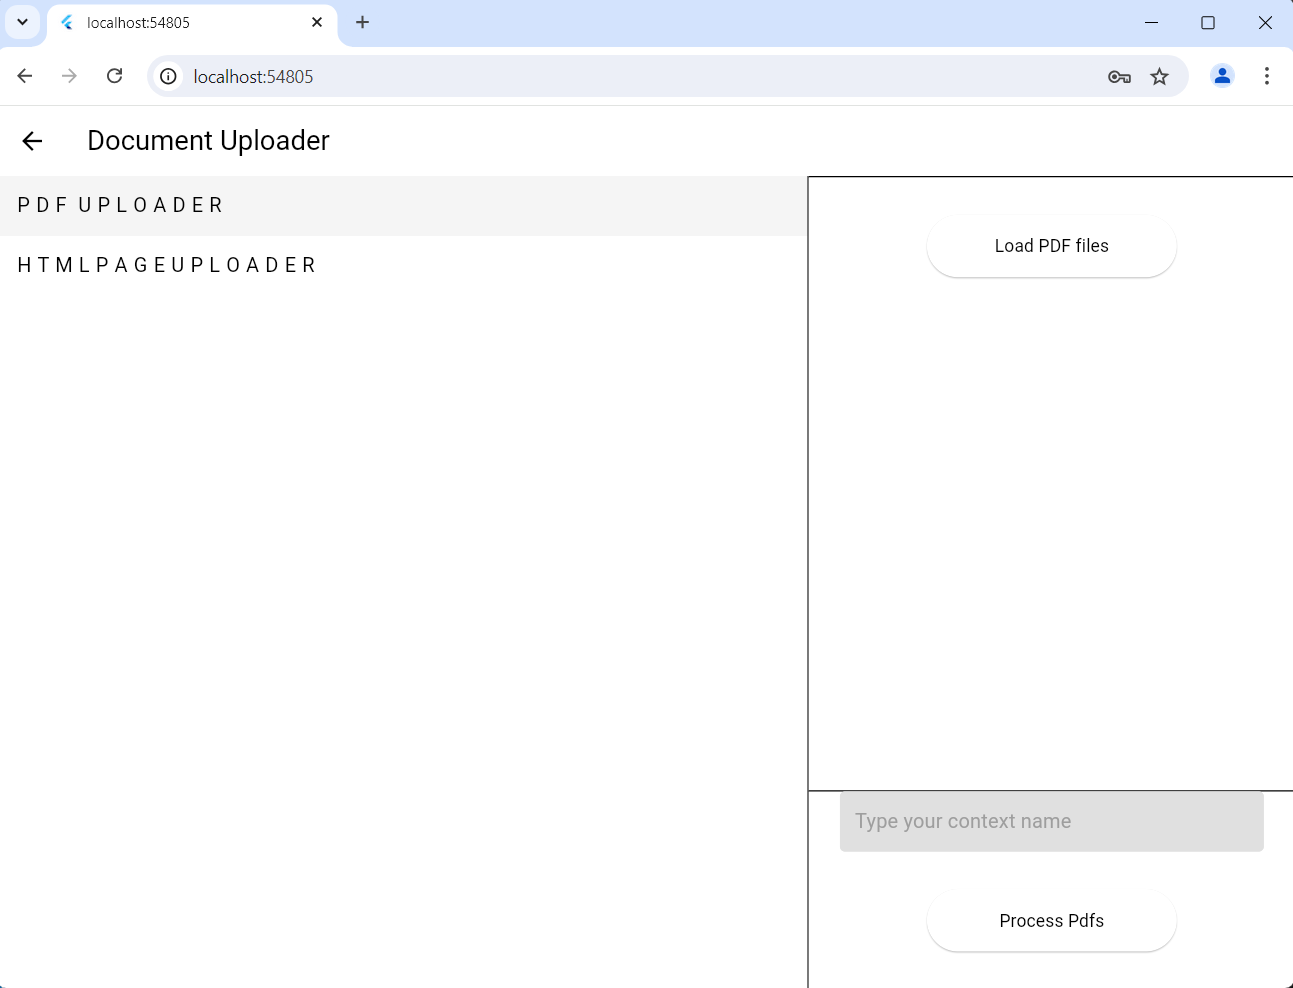
\includegraphics[width=0.45\linewidth]{Immagini/pdf_uploader_page.png}
		\caption{Pagina di caricamento di documenti PDF\newline}
		\label{fig:pdfs_page}
	\end{subfigure}%
	\begin{subfigure}{.5\textwidth}
		\centering
		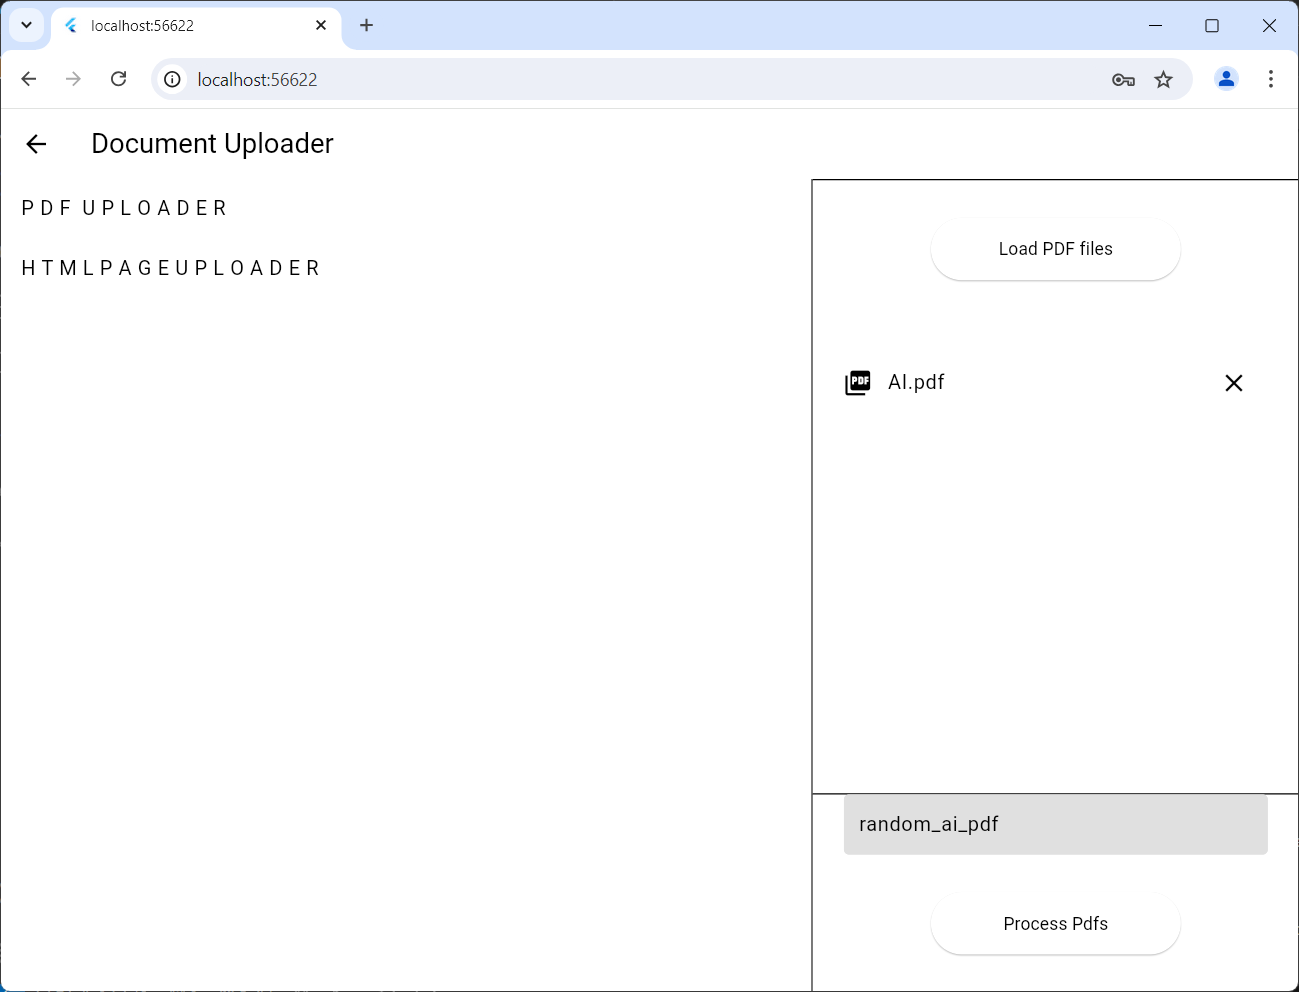
\includegraphics[width=0.45\linewidth]{Immagini/pdf_upload.png}
		\caption{Creazione di un nuovo contesto\newline}
		\label{fig:context-making}
	\end{subfigure}
	\begin{subfigure}{.5\textwidth}
		\centering
		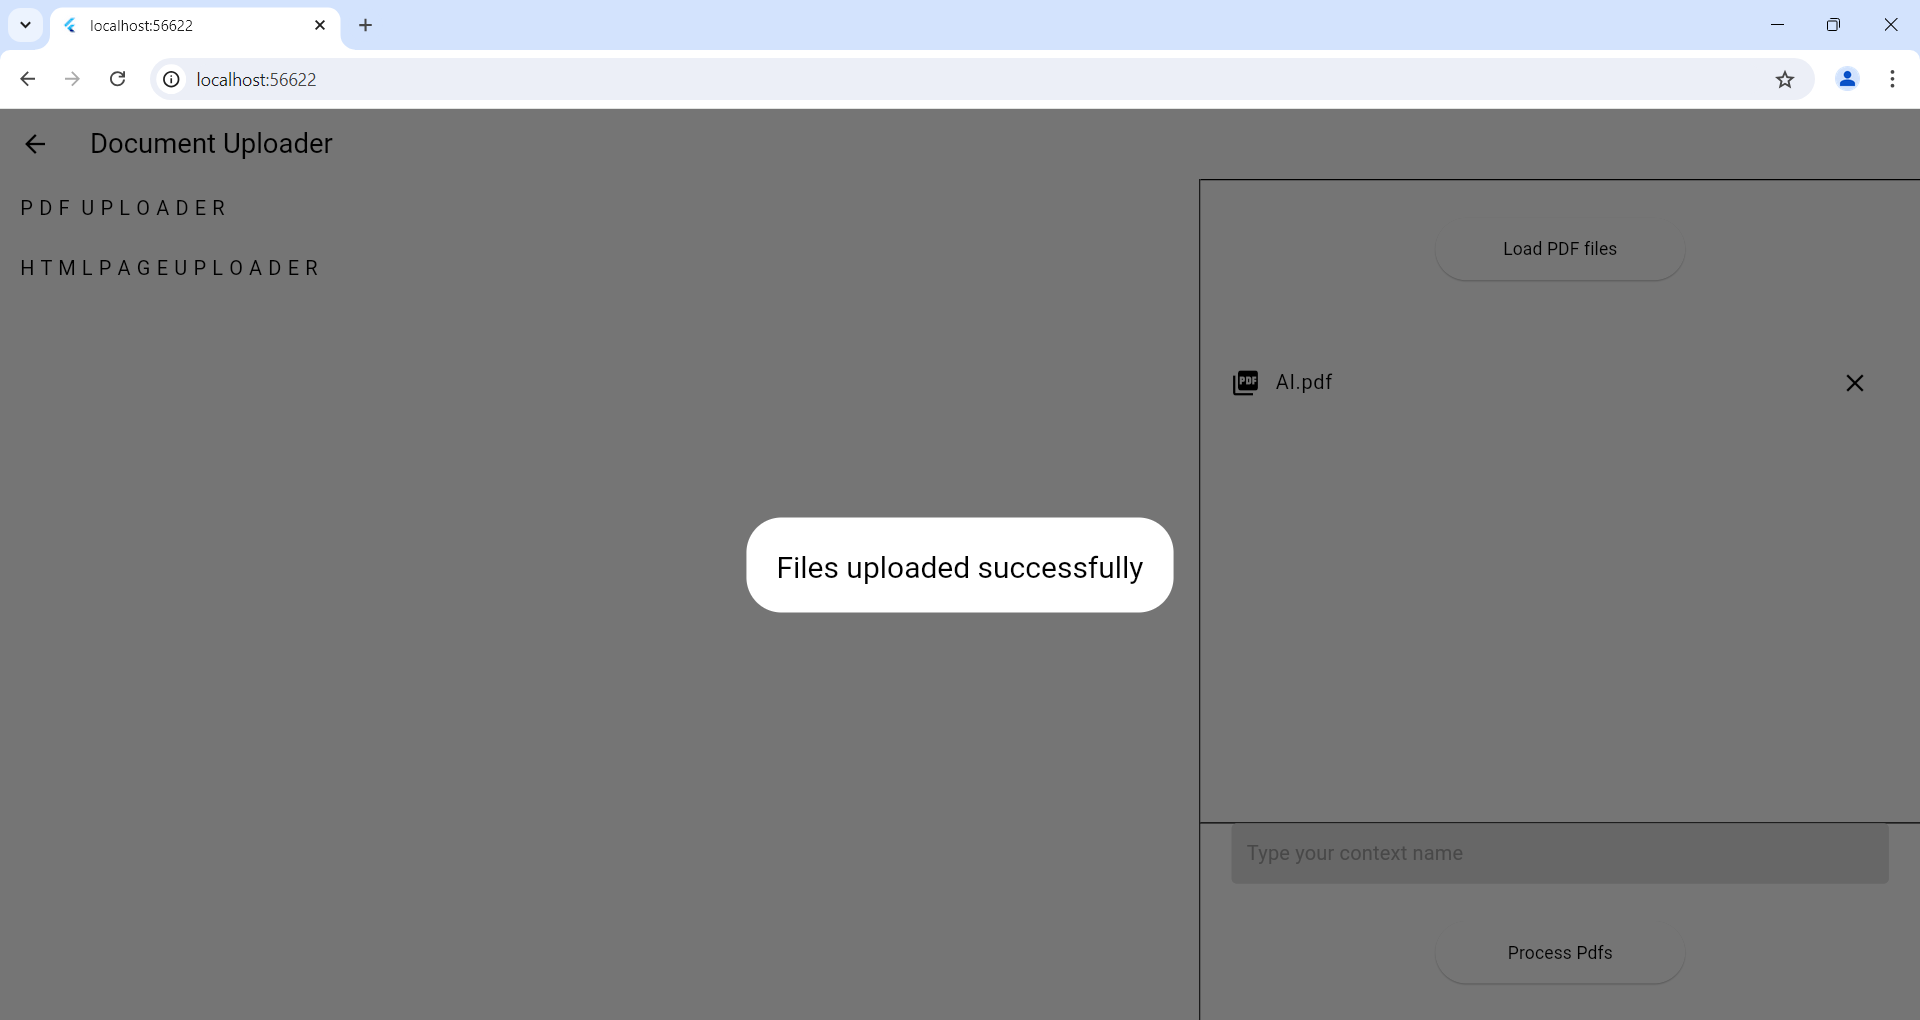
\includegraphics[width=0.45\linewidth]{Immagini/pdfs_successfully_upload.png}
		\caption{Notifica della creazione del nuovo contesto \newline}
		\label{fig:pdf_success}
	\end{subfigure}%
	\caption{Sezione per creare un nuovo contesto basato su documenti PDF}
\end{figure}

L'applicazione consente di creare un nuovo contesto utilizzando un insieme di file PDF, come illustrato nella figura \ref{fig:pdfs_context}, Inoltre, nella figura \ref{fig:pdf_removed}, è possibile osservare la funzionalità di rimozione di un documento tramite il pulsante "X" accanto al file. Questo pulsante elimina l'ultimo documento, rispetto a quanto mostrato nella figura \ref{fig:pdfs_context}.
\begin{figure}[H]
	\centering
        \begin{subfigure}{.5\textwidth}
		\centering
		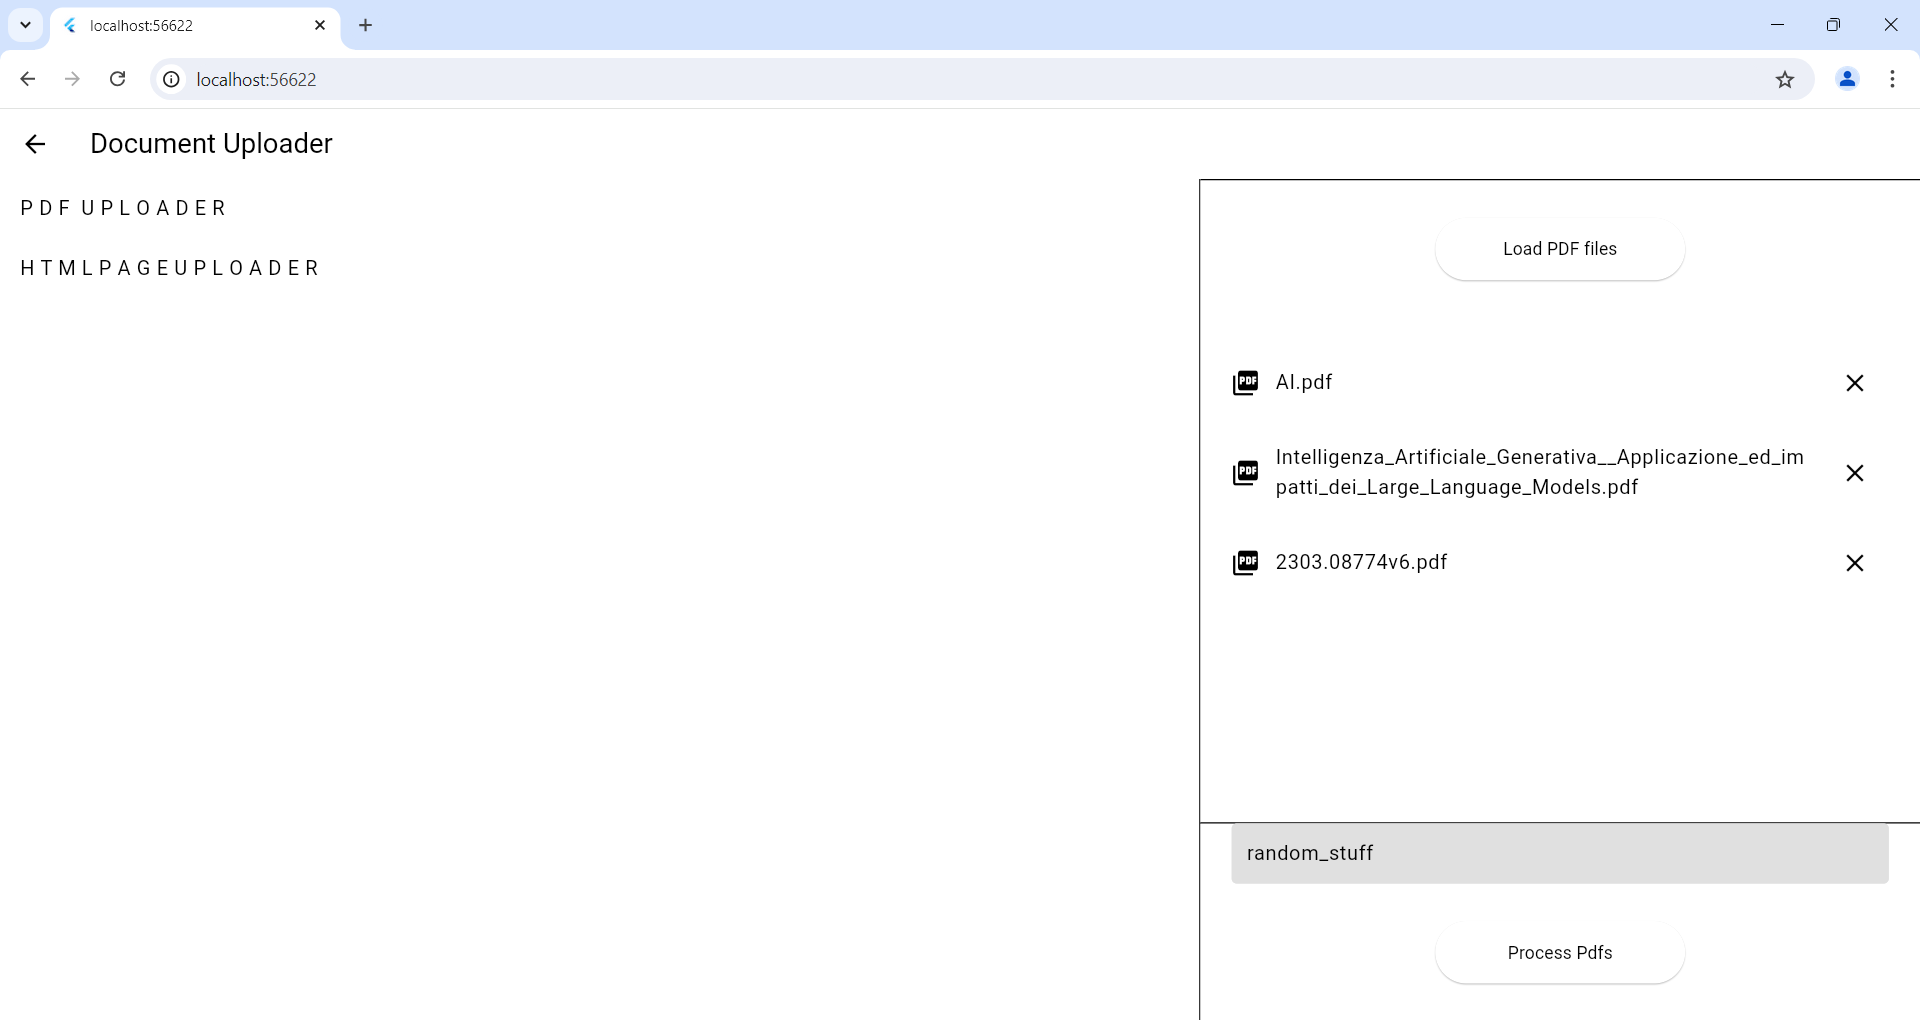
\includegraphics[width=0.45\linewidth]{Immagini/random_stuff.png}
		\caption{Creazione contesto con un'insieme di PDF\newline}
		\label{fig:pdfs_context}
	\end{subfigure}%
        \begin{subfigure}{.5\textwidth}
		\centering
		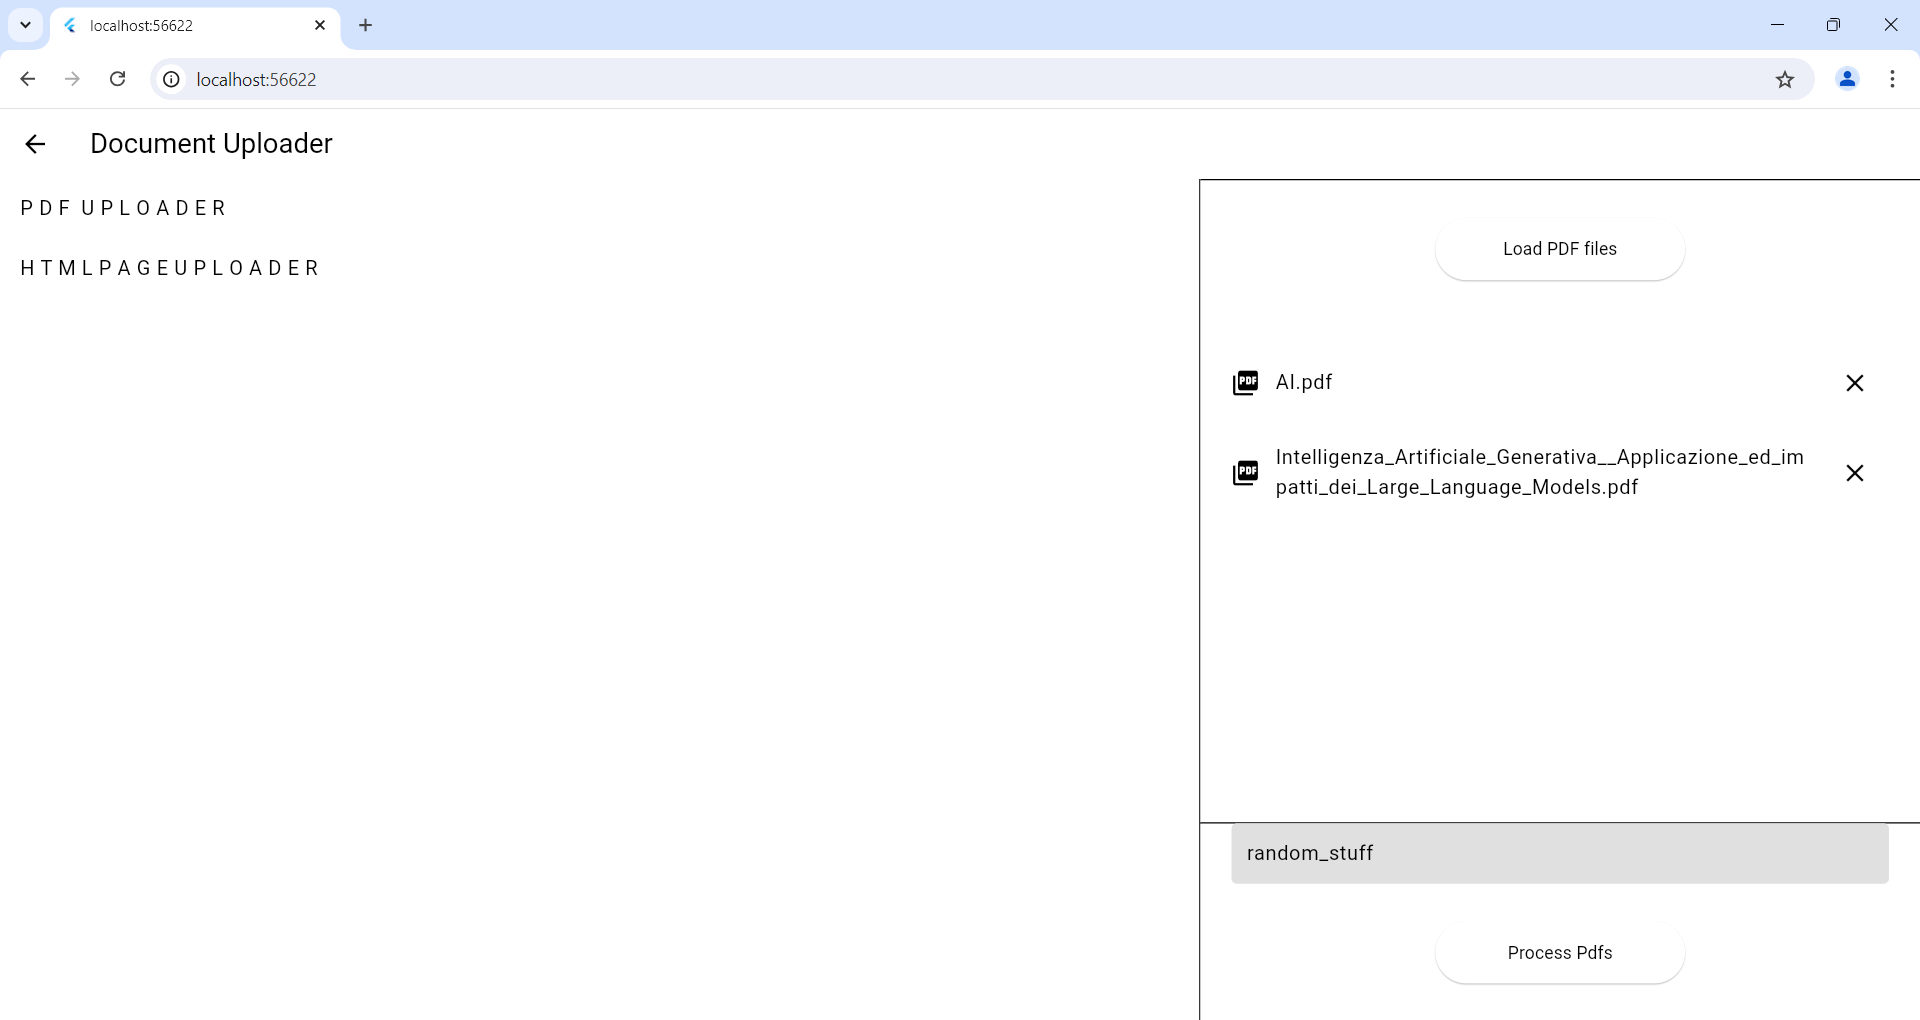
\includegraphics[width=0.45\linewidth]{Immagini/remove_one.png}
		\caption{Rimozione di un documento all'interno della lista\newline}
		\label{fig:pdf_removed}
	\end{subfigure}%
	\caption{Operazioni disponibili con la pagina di PDF Uploader}
\end{figure}

L'interfaccia per la creazione del contesto tramite pagine HTML è illustrata nella figura \ref{fig:html_section}. Essa include un campo per inserire gli URL delle pagine web, separati da un'interruzione di riga, e un pulsante per specificare il nome del contesto, come mostrato nella Figura \ref{fig:html_upload}.
Il processo per la creazione del contesto tramite pagine HTML è simile a quello per l'elaborazione dei PDF, con una sola differenza: una volta ricevuti gli URL, l'applicazione server estrae non solo le pagine HTML dai link forniti, ma anche le pagine figlie collegate all'interno di questi documenti, escludendo quelle che non appartengono al dominio specificato.

\begin{figure}[H]
	\centering
        \begin{subfigure}{.5\textwidth}
		\centering
		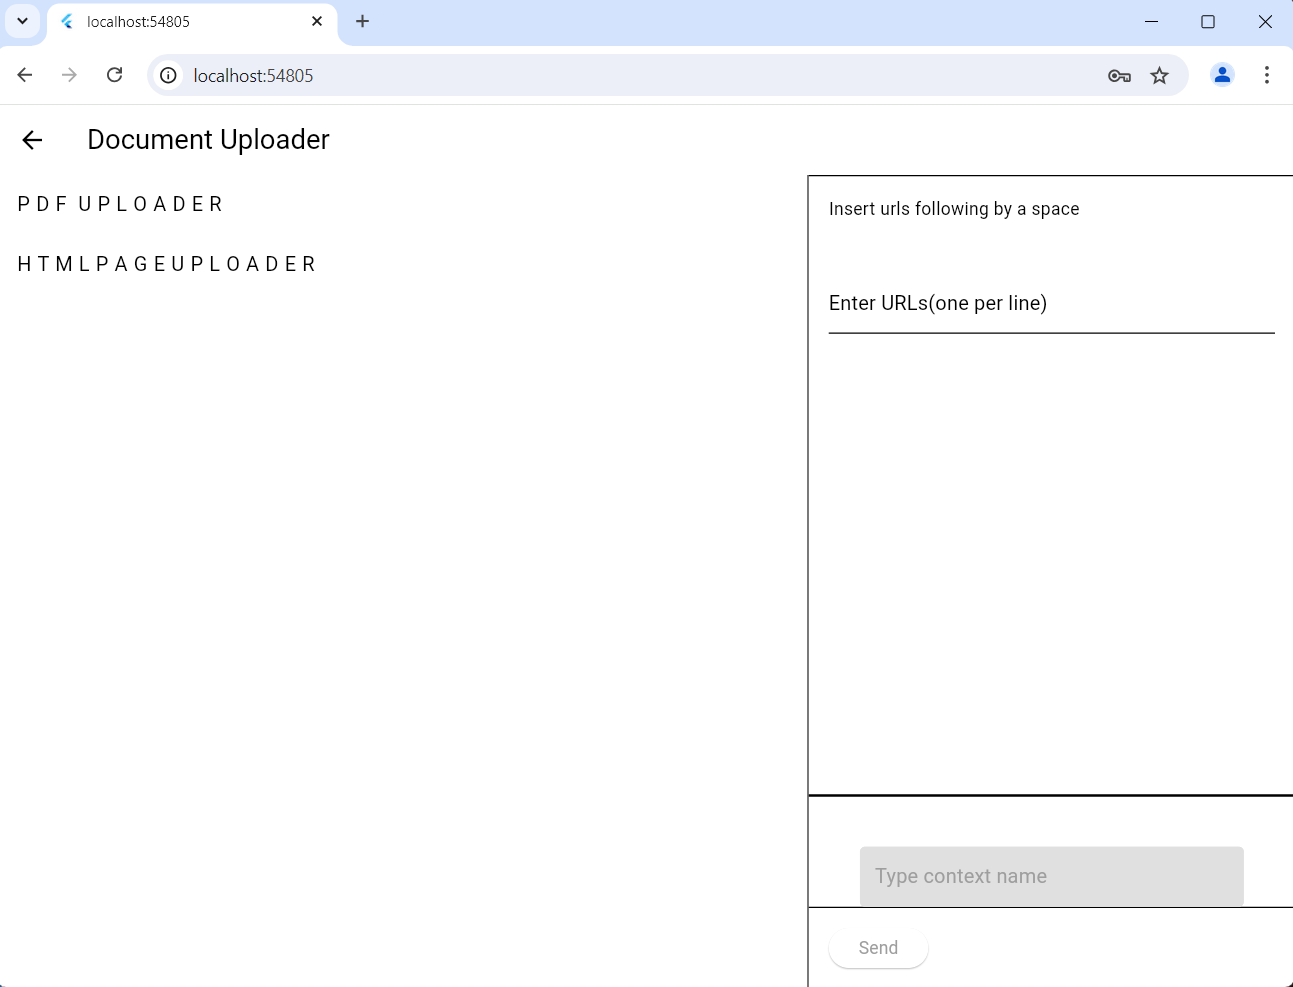
\includegraphics[width=0.45\linewidth]{Immagini/html_uploader_page.png}
		\caption{Sezione vuota per il caricamento di pagine HTML\newline}
		\label{fig:html_section}
	\end{subfigure}%
        \begin{subfigure}{.5\textwidth}
		\centering
		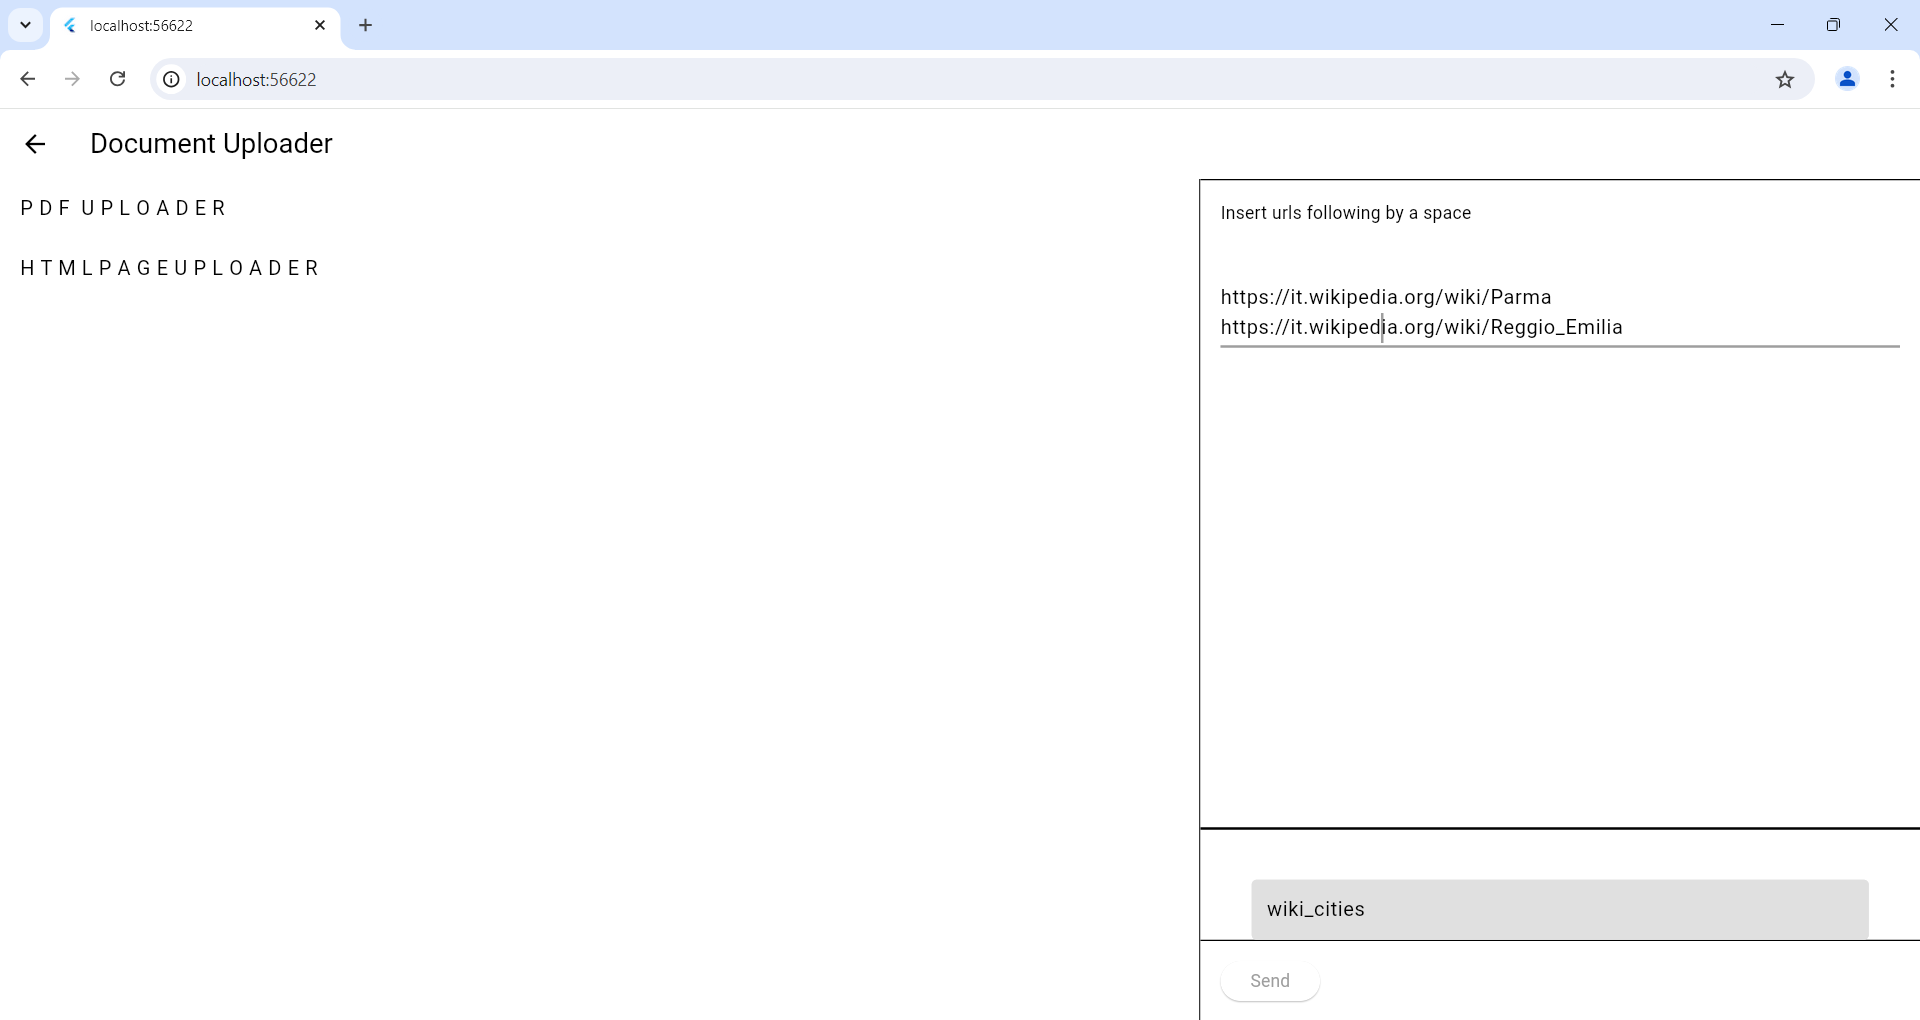
\includegraphics[width=0.45\linewidth]{Immagini/html_uploads.png}
		\caption{Rimozione di un documento all'interno della lista\newline}
		\label{fig:html_upload}
	\end{subfigure}%
	\caption{Sezione per il caricamento di Documenti HTML}
\end{figure}

\subsubsection{ChatBot}
La pagina del ChatBot consente all'utente di avviare una conversazione con un modello di linguaggio selezionando un contesto dalla sezione situata a destra, come mostrato nella Figura \ref{fig:chatbot}. Se la sezione è vuota, l'utente deve prima creare un contesto.

\begin{figure}[ht]
	\centering
	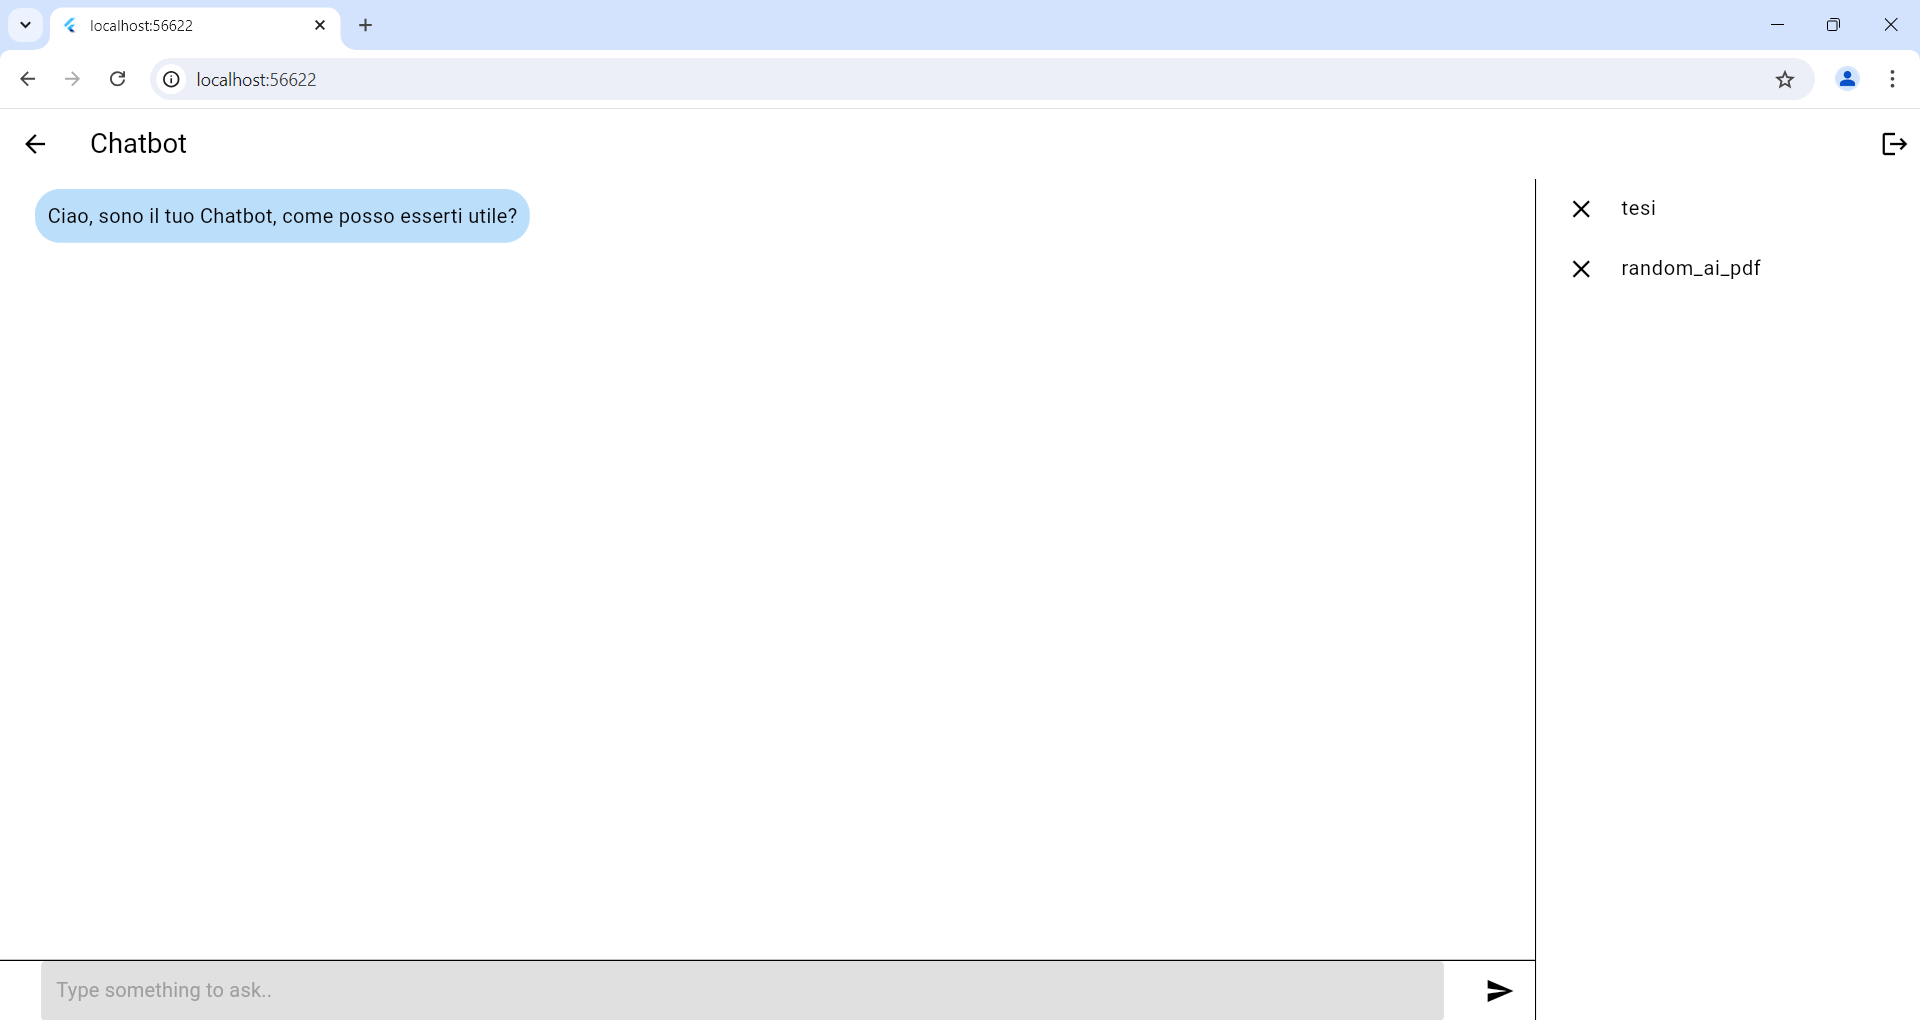
\includegraphics[width=0.3\textwidth]{Immagini/chatbot_page.png}
	\caption{Pagina del ChatBot dell'applicazione}
	\label{fig:chatbot}
\end{figure}
Una volta selezionato il contesto e inviata la domanda dall'utente, l'applicazione invia una richiesta HTTP al server, includendo la domanda e il contesto selezionato. Il server, tramite l'uso del retriever, recupera le informazioni pertinenti dal vettore di contesto presente nel database dell'utente e le integra nel prompt del modello di linguaggio. Successivamente, una volta generata la risposta, il server la invia all'applicazione. L'applicazione estrae quindi le informazioni dalla risposta HTTP e le visualizza a schermo tramite un messaggio per l'utente.
La Figura \ref{fig:chat} mostra alcune risposte generate dal modello di linguaggio e illustra il processo di comunicazione con il server.

\begin{figure}[H]
	\centering
        \begin{subfigure}{.5\textwidth}
		\centering
		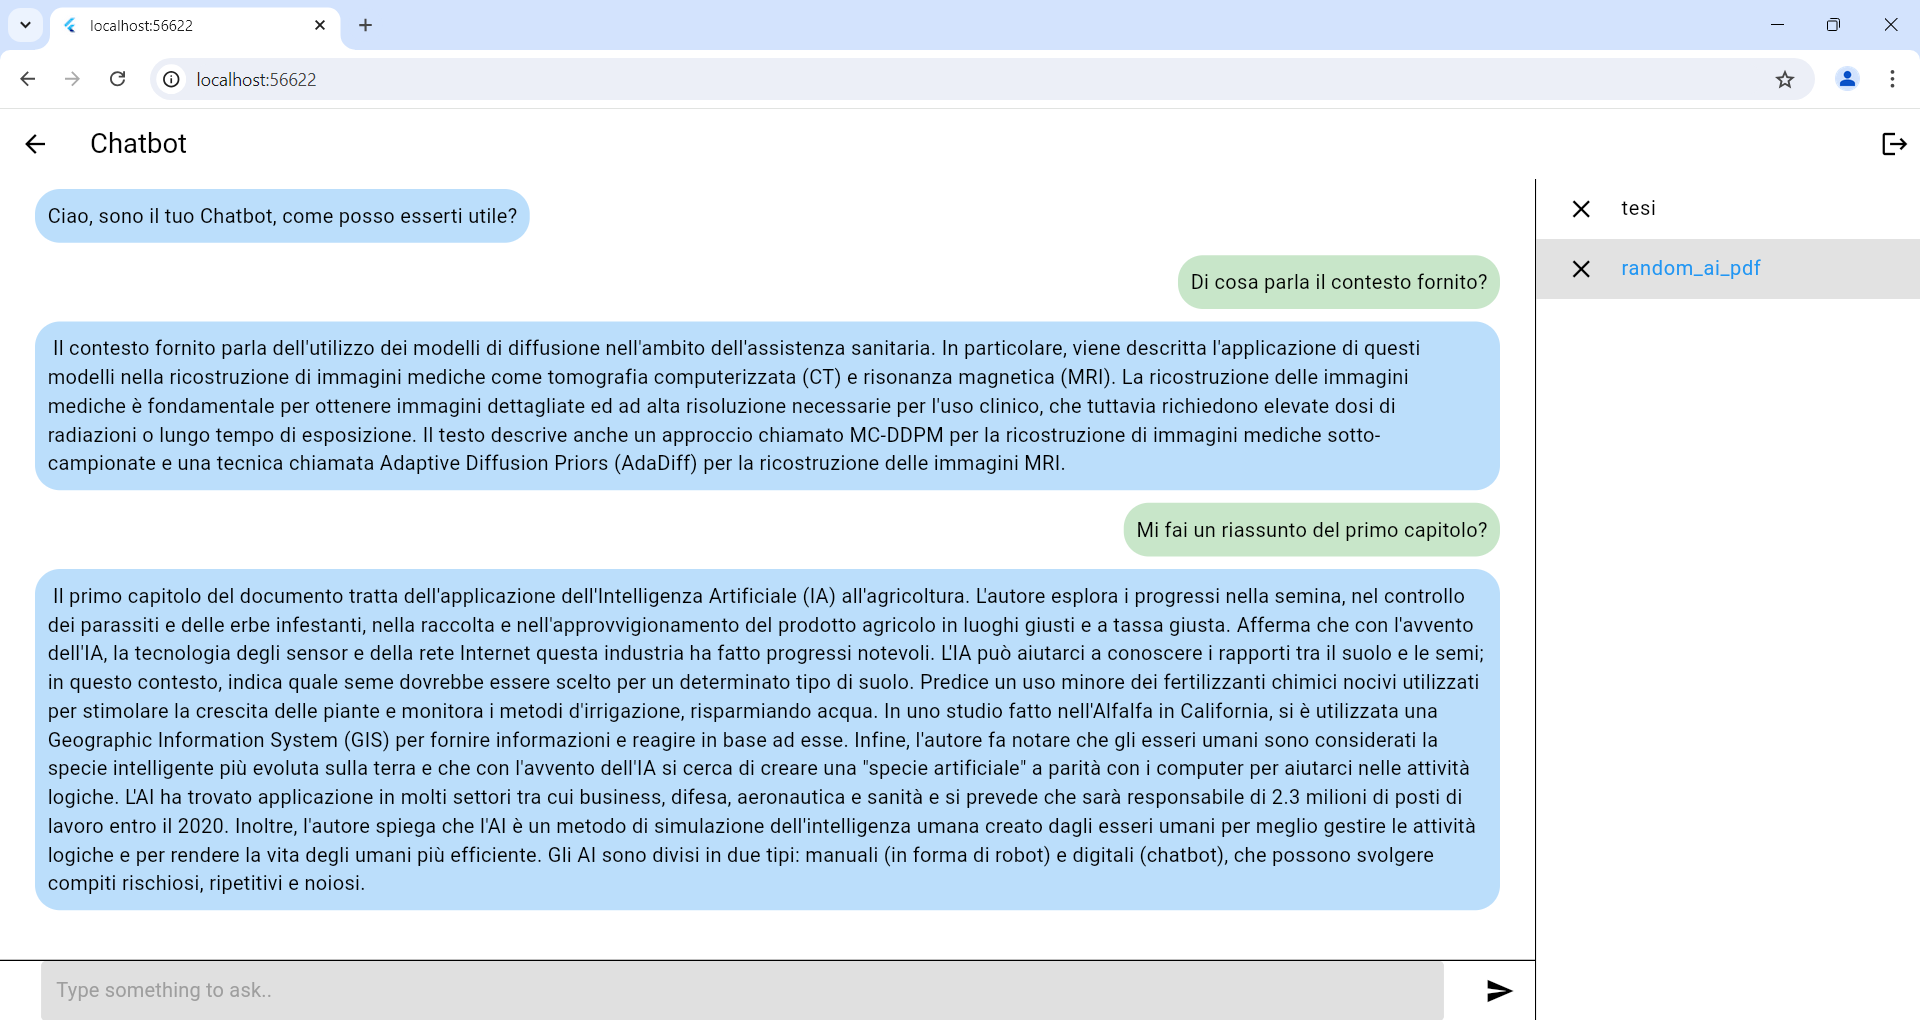
\includegraphics[width=0.45\linewidth]{Immagini/chat_example.png}
		\caption{Risposte generate dal modello linguaggio\newline}
	\end{subfigure}%
        \begin{subfigure}{.5\textwidth}
		\centering
		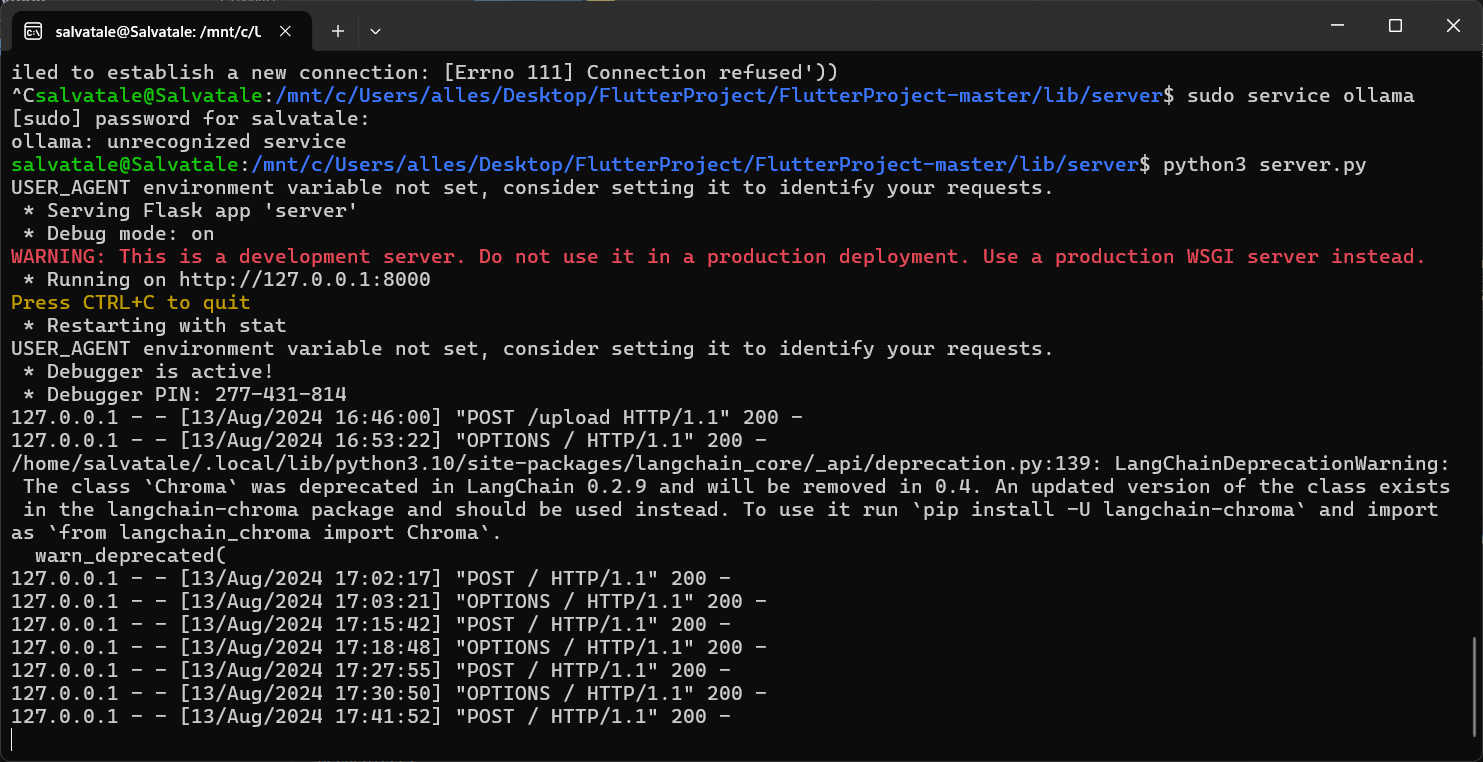
\includegraphics[width=0.45\linewidth]{Immagini/http_connections_during_conversation.png}
		\caption{Richieste HTTP generate dalla comunicazione tra server ed applicazione Flutter\newline}
	\end{subfigure}%
	\caption{Conversazione con il Chatbot}
        \label{fig:chat}
\end{figure}

\subsubsection{SpeechBot}
Lo speechbot permette all'utente di avere una conversazione vocale con il Bot come mostrato nella figura \ref{fig:speechbot}.
Il processo è simile a quello del ChatBot, ma con alcune differenze significative. Nel caso dello SpeechBot, l'utente deve registrare il proprio messaggio tramite microfono. L'applicazione converte l'audio in testo utilizzando la tecnologia Speech-to-Text. Successivamente, il messaggio ricevuto dal server viene convertito in audio tramite la tecnologia Text-to-Speech.
\begin{figure}[ht]
	\centering
	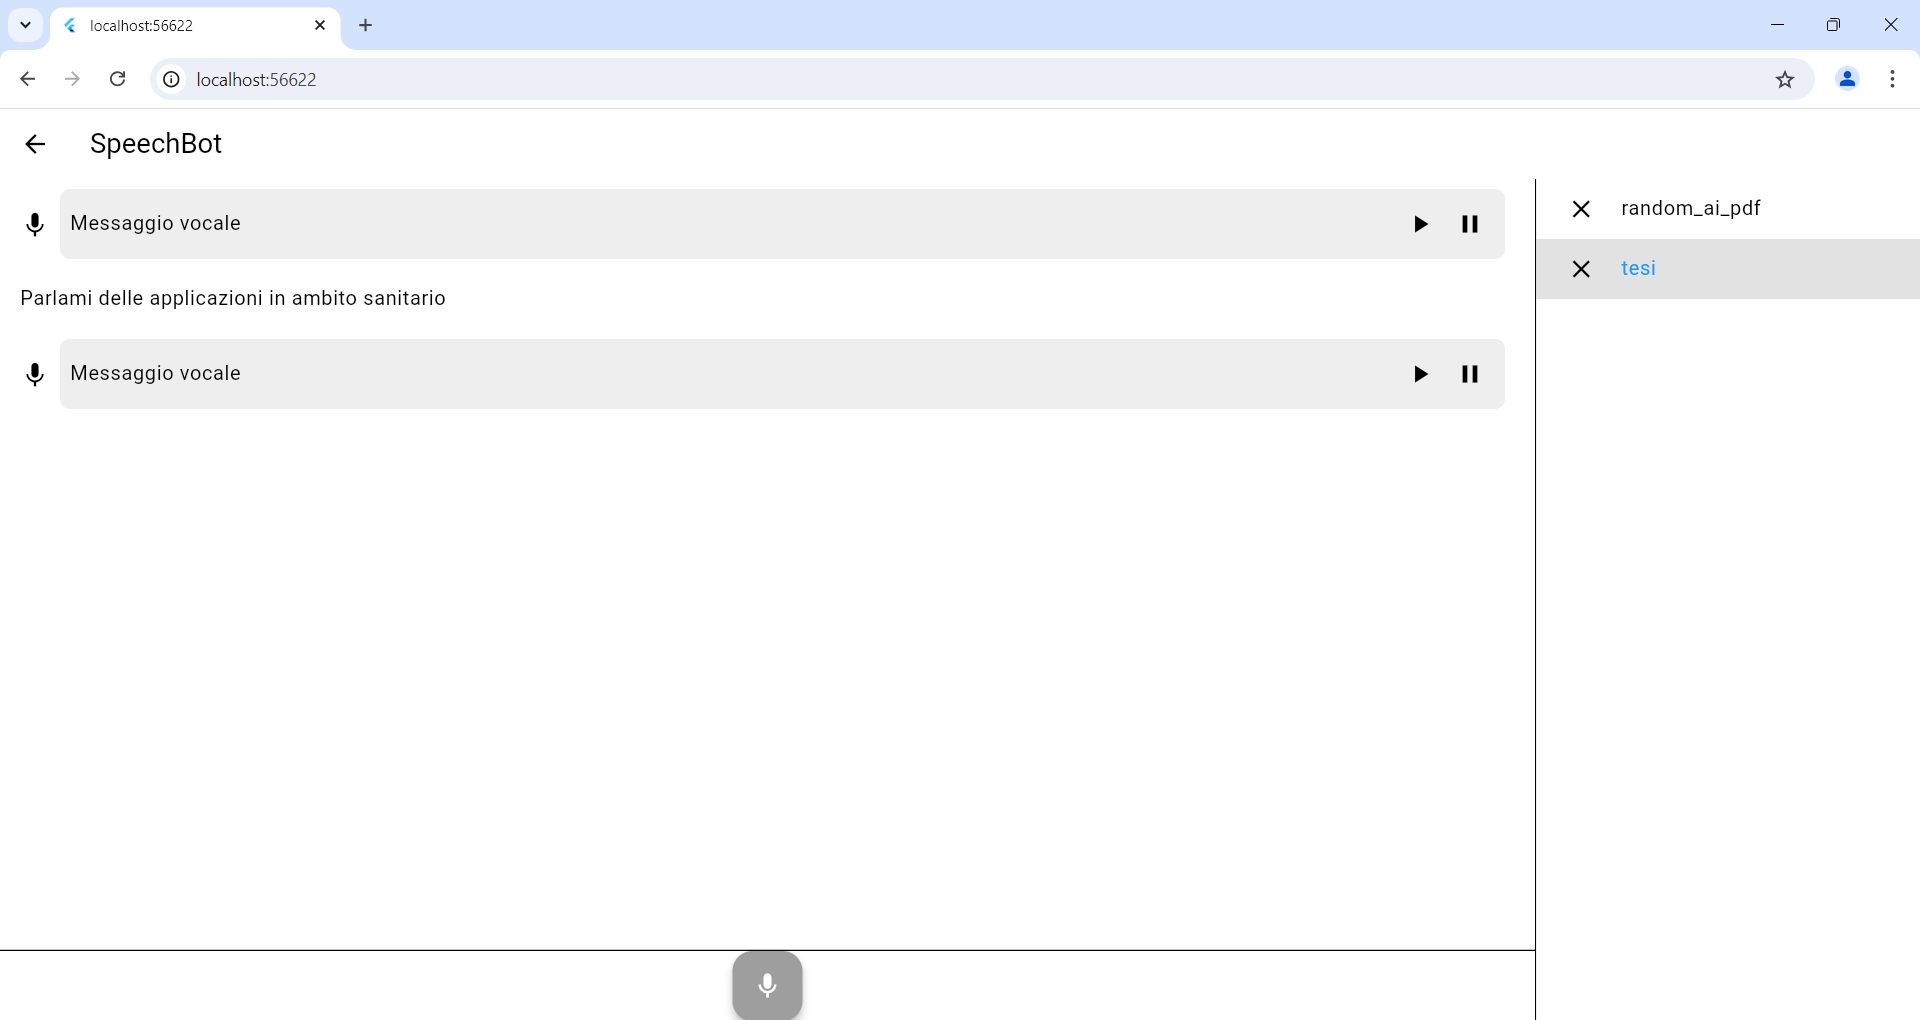
\includegraphics[width=0.3\textwidth]{Immagini/speechbot.png}
	\caption{Pagina dello SpeechBot dell'applicazione}
	\label{fig:speechbot}
\end{figure}

\section{Strumenti e tecnologie usate}

\subsection{Ollama}
Ollama è una piattaforma di supporto che funge da contenitore per modelli di linguaggio, analogamente a Docker per la gestione e distribuzione delle applicazioni. In particolare, Ollama consente di eseguire e gestire modelli di linguaggio all'interno di ambienti isolati e controllati, facilitando così la loro integrazione e distribuzione. La piattaforma offre anche la possibilità di scaricare i modelli in locale e di utilizzarli tramite codice Python.
Nell'ambito dell'applicazione, viene impiegato Mistral come modello di linguaggio di grandi dimensioni e nomic-embed-text come modello per l'embedding.

\subsection{Chroma}
Chroma è un database open-source ottimizzato per l'intelligenza artificiale, progettato per gestire e indicizzare grandi quantità di dati che le applicazioni AI utilizzano o generano. È costruito per essere altamente performante, scalabile e facile da integrare con altre applicazioni di machine learning o AI.
Nell'applicazione, Chroma fornisce i seguenti servizi: un database per l'archiviazione dei vettori relativi al contesto degli utenti, oltre a svolgere le funzioni di retriever e di generazione del vettore del contesto.

\subsection{Langchain}
LangChain è un framework progettato per facilitare la creazione di applicazioni basate su modelli di linguaggio, come GPT-4, attraverso la costruzione di catene di componenti interoperabili. Utilizzando il pacchetto LangChain in Python, è possibile sviluppare applicazioni avanzate basate su modelli di linguaggio sfruttando un'ampia gamma di funzionalità e componenti.
Nell'applicazione, LangChain fornisce l'integrazione di Ollama, Chroma e la gestione del prompt, consentendo di combinare questi elementi in un'architettura RAG. Questo permette al sistema di rispondere alle domande in modo contestuale, attingendo sia ai modelli di linguaggio che ai dati specifici degli utenti.

\subsection{Text-to-Speech}
Il pacchetto Flutter utilizzato per convertire il testo in audio all'interno dell'applicazione è 'flutter\_tts'. Questo pacchetto offre funzionalità di sintesi vocale, permettendo all'applicazione di trasformare il testo in audio in modo fluido e integrato.

\subsection{Speech-To-Text}
Il pacchetto Flutter utilizzato per convertire l'audio in testo all'interno dell'applicazione è speech\_to\_text. Questo pacchetto fornisce funzionalità di riconoscimento vocale, permettendo all'applicazione di trascrivere l'audio in testo in modo efficace e preciso.

\subsection{Flask}
Flask è un framework web leggero per Python, progettato per facilitare la creazione di applicazioni web in modo rapido e semplice, mantenendo al contempo la flessibilità necessaria per gestire applicazioni complesse.
All'interno dell'applicazione viene utilizzato per ricevere ed inviare richieste HTTP tra Flutter ed il server.

\section{Prestazioni Chatbot ed obiettivi futuri}

\subsection{Performance}
Il Chatbot, in termini di prestazioni, risulta mediocre. Sebbene le risposte siano per lo più corrette, sono spesso molto sintetiche e talvolta il sistema fatica a comprendere le domande. Inoltre, i tempi di generazione sono piuttosto lunghi, variando in base all'architettura su cui è in esecuzione. 
Quando il Chatbot opera su una GPU di basso livello, la generazione delle risposte richiede circa 1-2 minuti. Questo suggerisce che, se gestito con una GPU di buona qualità, la generazione delle risposte potrebbe avvenire in modo quasi istantaneo, migliorando notevolmente le prestazioni complessive del sistema.
Considerando i tempi di attesa significativamente lunghi quando si utilizza solo la CPU, è stata aggiunta la possibilità di implementare il MailBot. Questo permette di inviare le risposte via email, in modo che l'utente non debba attendere il completamento della generazione direttamente nell'interfaccia, migliorando l'esperienza complessiva.
Per quanto riguarda la creazione del vettore del contesto, anche con l'uso di GPU, questo processo può risultare estremamente lungo. Sebbene non rappresenti un problema sostanziale per l'utente, poiché il processo può essere gestito in background, costituisce un limite significativo per le risorse computazionali. Infatti, il lungo tempo di elaborazione potrebbe rallentare altri processi in esecuzione, influenzando negativamente le prestazioni complessive del sistema.

\subsection{Obiettivi futuri e possinili applicazioni}
Per migliorare il Chatbot e ampliare le sue capacità, si potrebbero considerare diverse nuove funzionalità. Una delle principali aggiunte sarebbe la possibilità per l'utente di scegliere la lingua di generazione delle risposte o di selezionare il modello di linguaggio preferito tra quelli disponibili. Questo permetterebbe una personalizzazione maggiore e una maggiore flessibilità nell'interazione con il sistema.
Un'altra modifica che l'utente può compiere potrebbe essere la capacità di abbassare il parametro "temperature" che permette al modello di aumentare la serietà delle risposte tanto più alto il valore, questo darebbe la capacità al modello di generare risposte fantasiose quando parla con un bambino.
Inoltre, sarebbe utile offrire agli utenti la possibilità di gestire i propri contesti con maggiore facilità. Attualmente, l'applicazione consente di creare un contesto tramite la pagina del "Doc Uploader" e di eliminarlo tramite un semplice clic sulla "X" accanto al contesto nella sezione a destra delle pagine di Chat. Questa funzionalità potrebbe essere ulteriormente affinata per una gestione più intuitiva e completa dei contesti.
Un'altra possibile implementazione è un'interfaccia nella pagina di "SpeechBot" che simuli una chiamata vocale, offrendo un'interazione più naturale e immediata tra l'utente e il Chatbot. Questa funzionalità potrebbe migliorare l'esperienza utente, rendendo la comunicazione più fluida e coinvolgente.
\newline

Il chatbot potrebbe essere utilizzato per l'elaborazione di documenti e per la specializzazione in determinati contesti, rivelandosi un supporto prezioso per le persone in diversi ambiti. Ad esempio, potrebbe essere impiegato in un museo per rispondere a domande dei turisti riguardanti la storia delle opere e delle sculture, offrendo informazioni dettagliate e contestualizzate. In ambito educativo, potrebbe assistere gli studenti nella preparazione di esami, permettendo loro di salvare contesti specifici come "esame", formulare domande ed esercizi, e verificare le risposte ottenute. Inoltre, il chatbot potrebbe rappresentare un aiuto significativo per i professori, facilitando la generazione di domande casuali per esami o esercitazioni e migliorando l'efficienza nella preparazione e gestione delle prove. Implementando tali funzionalità, il chatbot diventa uno strumento estremamente versatile e utile in una varietà di contesti.
Gli usi finora elencati sono solo alcune delle possibili applicazioni del chatbot. A seconda delle esigenze specifiche dell'utente, il chatbot può essere adattato e personalizzato per soddisfare una vasta gamma di scenari e requisiti. La sua versatilità consente di ottimizzare le sue funzionalità per rispondere a necessità diverse e variabili.
